\documentclass[a4paper]{article}

\def\npart {IB}
\def\nterm {Michaelmas}
\def\nyear {2015}
\def\nlecturer {D. B. Skinner}
\def\ncourse {Methods}
\def\nofficial {http://www.damtp.cam.ac.uk/user/dbs26/1Bmethods.html}
\def\nlectures {MWF.9}
\def\nnotready {}

% Imports
\ifx \nextra \undefined
  \usepackage[pdftex,
    hidelinks,
    pdfauthor={Dexter Chua},
    pdfsubject={Cambridge Maths Notes: Part \npart\ - \ncourse},
    pdftitle={Part \npart\ - \ncourse},
  pdfkeywords={Cambridge Mathematics Maths Math \npart\ \nterm\ \nyear\ \ncourse}]{hyperref}
  \title{Part \npart\ - \ncourse}
\else
  \usepackage[pdftex,
    hidelinks,
    pdfauthor={Dexter Chua},
    pdfsubject={Cambridge Maths Notes: Part \npart\ - \ncourse\ (\nextra)},
    pdftitle={Part \npart\ - \ncourse\ (\nextra)},
  pdfkeywords={Cambridge Mathematics Maths Math \npart\ \nterm\ \nyear\ \ncourse\ \nextra}]{hyperref}

  \title{Part \npart\ - \ncourse \\ {\Large \nextra}}
\fi

\author{Lectured by \nlecturer \\\small Notes taken by Dexter Chua}
\date{\nterm\ \nyear}

\usepackage{alltt}
\usepackage{amsfonts}
\usepackage{amsmath}
\usepackage{amssymb}
\usepackage{amsthm}
\usepackage{booktabs}
\usepackage{caption}
\usepackage{enumitem}
\usepackage{fancyhdr}
\usepackage{graphicx}
\usepackage{mathtools}
\usepackage{microtype}
\usepackage{multirow}
\usepackage{pdflscape}
\usepackage{pgfplots}
\usepackage{siunitx}
\usepackage{tabularx}
\usepackage{tikz}
\usepackage{tkz-euclide}
\usepackage[normalem]{ulem}
\usepackage[all]{xy}

\pgfplotsset{compat=1.12}

\pagestyle{fancyplain}
\lhead{\emph{\nouppercase{\leftmark}}}
\ifx \nextra \undefined
  \rhead{
    \ifnum\thepage=1
    \else
      \npart\ \ncourse
    \fi}
\else
  \rhead{
    \ifnum\thepage=1
    \else
      \npart\ \ncourse\ (\nextra)
    \fi}
\fi
\usetikzlibrary{arrows}
\usetikzlibrary{decorations.markings}
\usetikzlibrary{decorations.pathmorphing}
\usetikzlibrary{positioning}
\usetikzlibrary{fadings}
\usetikzlibrary{intersections}
\usetikzlibrary{cd}

\newcommand*{\Cdot}{\raisebox{-0.25ex}{\scalebox{1.5}{$\cdot$}}}
\newcommand {\pd}[2][ ]{
  \ifx #1 { }
    \frac{\partial}{\partial #2}
  \else
    \frac{\partial^{#1}}{\partial #2^{#1}}
  \fi
}

% Theorems
\theoremstyle{definition}
\newtheorem*{aim}{Aim}
\newtheorem*{axiom}{Axiom}
\newtheorem*{claim}{Claim}
\newtheorem*{cor}{Corollary}
\newtheorem*{defi}{Definition}
\newtheorem*{eg}{Example}
\newtheorem*{fact}{Fact}
\newtheorem*{law}{Law}
\newtheorem*{lemma}{Lemma}
\newtheorem*{notation}{Notation}
\newtheorem*{prop}{Proposition}
\newtheorem*{thm}{Theorem}

\renewcommand{\labelitemi}{--}
\renewcommand{\labelitemii}{$\circ$}
\renewcommand{\labelenumi}{(\roman{*})}

\let\stdsection\section
\renewcommand\section{\newpage\stdsection}

% Strike through
\def\st{\bgroup \ULdepth=-.55ex \ULset}

% Maths symbols
\newcommand{\bra}{\langle}
\newcommand{\ket}{\rangle}

\newcommand{\N}{\mathbb{N}}
\newcommand{\Z}{\mathbb{Z}}
\newcommand{\Q}{\mathbb{Q}}
\renewcommand{\H}{\mathbb{H}}
\newcommand{\R}{\mathbb{R}}
\newcommand{\C}{\mathbb{C}}
\newcommand{\Prob}{\mathbb{P}}
\renewcommand{\P}{\mathbb{P}}
\newcommand{\E}{\mathbb{E}}
\newcommand{\F}{\mathbb{F}}
\newcommand{\cU}{\mathcal{U}}
\newcommand{\RP}{\mathbb{RP}}
\newcommand{\CP}{\mathbb{CP}}

\newcommand{\ph}{\,\cdot\,}

\DeclareMathOperator{\sech}{sech}
\DeclareMathOperator{\cosech}{cosech}
\DeclareMathOperator{\cosec}{cosec}

\DeclareMathOperator{\covol}{covol}
\DeclareMathOperator{\vol}{vol}

\let\Im\relax
\let\Re\relax
\DeclareMathOperator{\Im}{Im}
\DeclareMathOperator{\Re}{Re}
\DeclareMathOperator{\im}{im}
\DeclareMathOperator{\image}{image}
\DeclareMathOperator{\Ann}{Ann}

\DeclareMathOperator*{\res}{res}
\DeclareMathOperator{\Res}{Res}
\DeclareMathOperator{\Ind}{Ind}

\DeclareMathOperator{\tr}{tr}
\DeclareMathOperator{\diag}{diag}
\DeclareMathOperator{\rank}{rank}
\DeclareMathOperator{\card}{card}
\DeclareMathOperator{\spn}{span}
\DeclareMathOperator{\adj}{adj}

\DeclareMathOperator{\erf}{erf}
\DeclareMathOperator{\erfc}{erfc}

\DeclareMathOperator{\ord}{ord}
\DeclareMathOperator{\Sym}{Sym}

\DeclareMathOperator{\sgn}{sgn}
\DeclareMathOperator{\orb}{orb}
\DeclareMathOperator{\stab}{stab}
\DeclareMathOperator{\ccl}{ccl}

\DeclareMathOperator{\lcm}{lcm}
\DeclareMathOperator{\hcf}{hcf}

\DeclareMathOperator{\Int}{Int}
\DeclareMathOperator{\id}{id}

\DeclareMathOperator{\betaD}{beta}
\DeclareMathOperator{\gammaD}{gamma}
\DeclareMathOperator{\Poisson}{Poisson}
\DeclareMathOperator{\binomial}{binomial}
\DeclareMathOperator{\multinomial}{multinomial}
\DeclareMathOperator{\Bernoulli}{Bernoulli}
\DeclareMathOperator{\like}{like}

\DeclareMathOperator{\var}{var}
\DeclareMathOperator{\cov}{cov}
\DeclareMathOperator{\bias}{bias}
\DeclareMathOperator{\mse}{mse}
\DeclareMathOperator{\corr}{corr}

\DeclareMathOperator{\otp}{otp}
\DeclareMathOperator{\dom}{dom}

\DeclareMathOperator{\Root}{Root}
\DeclareMathOperator{\supp}{supp}
\DeclareMathOperator{\rel}{rel}
\DeclareMathOperator{\Hom}{Hom}
\DeclareMathOperator{\Aut}{Aut}
\DeclareMathOperator{\Gal}{Gal}
\DeclareMathOperator{\Mat}{Mat}
\DeclareMathOperator{\End}{End}
\DeclareMathOperator{\Char}{char}
\DeclareMathOperator{\ev}{ev}
\DeclareMathOperator{\St}{St}
\DeclareMathOperator{\Lk}{Lk}
\DeclareMathOperator{\disc}{disc}
\DeclareMathOperator{\Isom}{Isom}
\DeclareMathOperator{\length}{length}
\DeclareMathOperator{\energy}{energy}
\DeclareMathOperator{\area}{area}
\DeclareMathOperator{\Syl}{Syl}
\DeclareMathOperator{\cl}{cl}
\DeclareMathOperator{\fix}{fix}

\newcommand{\GL}{\mathrm{GL}}
\newcommand{\SL}{\mathrm{SL}}
\newcommand{\PGL}{\mathrm{PGL}}
\newcommand{\PSL}{\mathrm{PSL}}
\newcommand{\PSU}{\mathrm{PSU}}
\newcommand{\Or}{\mathrm{O}}
\newcommand{\SO}{\mathrm{SO}}
\newcommand{\U}{\mathrm{U}}
\newcommand{\SU}{\mathrm{SU}}

\renewcommand{\d}{\mathrm{d}}
\newcommand{\D}{\mathrm{D}}

\tikzset{->/.style = {decoration={markings,
                                  mark=at position 1 with {\arrow[scale=2]{latex'}}},
                      postaction={decorate}}}
\tikzset{<-/.style = {decoration={markings,
                                  mark=at position 0 with {\arrowreversed[scale=2]{latex'}}},
                      postaction={decorate}}}
\tikzset{<->/.style = {decoration={markings,
                                   mark=at position 0 with {\arrowreversed[scale=2]{latex'}},
                                   mark=at position 1 with {\arrow[scale=2]{latex'}}},
                       postaction={decorate}}}
\tikzset{->-/.style = {decoration={markings,
                                   mark=at position #1 with {\arrow[scale=2]{latex'}}},
                       postaction={decorate}}}
\tikzset{-<-/.style = {decoration={markings,
                                   mark=at position #1 with {\arrowreversed[scale=2]{latex'}}},
                       postaction={decorate}}}

\tikzset{circ/.style = {fill, circle, inner sep = 0, minimum size = 3}}
\tikzset{mstate/.style={circle, draw, blue, text=black, minimum width=0.7cm}}

\definecolor{mblue}{rgb}{0.2, 0.3, 0.8}
\definecolor{morange}{rgb}{1, 0.5, 0}
\definecolor{mgreen}{rgb}{0.1, 0.4, 0.2}
\definecolor{mred}{rgb}{0.5, 0, 0}

\def\drawcirculararc(#1,#2)(#3,#4)(#5,#6){%
    \pgfmathsetmacro\cA{(#1*#1+#2*#2-#3*#3-#4*#4)/2}%
    \pgfmathsetmacro\cB{(#1*#1+#2*#2-#5*#5-#6*#6)/2}%
    \pgfmathsetmacro\cy{(\cB*(#1-#3)-\cA*(#1-#5))/%
                        ((#2-#6)*(#1-#3)-(#2-#4)*(#1-#5))}%
    \pgfmathsetmacro\cx{(\cA-\cy*(#2-#4))/(#1-#3)}%
    \pgfmathsetmacro\cr{sqrt((#1-\cx)*(#1-\cx)+(#2-\cy)*(#2-\cy))}%
    \pgfmathsetmacro\cA{atan2(#2-\cy,#1-\cx)}%
    \pgfmathsetmacro\cB{atan2(#6-\cy,#5-\cx)}%
    \pgfmathparse{\cB<\cA}%
    \ifnum\pgfmathresult=1
        \pgfmathsetmacro\cB{\cB+360}%
    \fi
    \draw (#1,#2) arc (\cA:\cB:\cr);%
}
\newcommand\getCoord[3]{\newdimen{#1}\newdimen{#2}\pgfextractx{#1}{\pgfpointanchor{#3}{center}}\pgfextracty{#2}{\pgfpointanchor{#3}{center}}}

\def\Xint#1{\mathchoice
   {\XXint\displaystyle\textstyle{#1}}%
   {\XXint\textstyle\scriptstyle{#1}}%
   {\XXint\scriptstyle\scriptscriptstyle{#1}}%
   {\XXint\scriptscriptstyle\scriptscriptstyle{#1}}%
   \!\int}
\def\XXint#1#2#3{{\setbox0=\hbox{$#1{#2#3}{\int}$}
     \vcenter{\hbox{$#2#3$}}\kern-.5\wd0}}
\def\ddashint{\Xint=}
\def\dashint{\Xint-}


\begin{document}
\maketitle
{\small
\noindent\textbf{Self-adjoint ODEs}\\
Periodic functions. Fourier series: definition and simple properties; Parseval's theorem. Equations of second order. Self-adjoint differential operators. The Sturm-Liouville equation; eigenfunctions and eigenvalues; reality of eigenvalues and orthogonality of eigenfunctions; eigenfunction expansions (Fourier series as prototype), approximation in mean square, statement of completeness.\hspace*{\fill} [5]

\vspace{10pt}
\noindent\textbf{PDEs on bounded domains: separation of variables}\\
Physical basis of Laplace's equation, the wave equation and the diffusion equation. General method of separation of variables in Cartesian, cylindrical and spherical coordinates. Legendre's equation: derivation, solutions including explicit forms of $P_0$, $P_1$ and $P_2$, orthogonality. Bessel's equation of integer order as an example of a self-adjoint eigenvalue problem with non-trivial weight.

\vspace{5pt}
\noindent Examples including potentials on rectangular and circular domains and on a spherical domain (axisymmetric case only), waves on a finite string and heat flow down a semi-infinite rod.\hspace*{\fill} [5]

\vspace{10pt}
\noindent\textbf{Inhomogeneous ODEs: Green's functions}\\
Properties of the Dirac delta function. Initial value problems and forced problems with two fixed end points; solution using Green's functions. Eigenfunction expansions of the delta function and Green's functions.\hspace*{\fill} [4]

\vspace{10pt}
\noindent\textbf{Fourier transforms}\\
Fourier transforms: definition and simple properties; inversion and convolution theorems. The discrete Fourier transform. Examples of application to linear systems. Relationship of transfer function to Green's function for initial value problems.\hspace*{\fill} [4]

\vspace{10pt}
\noindent\textbf{PDEs on unbounded domains}\\
Classification of PDEs in two independent variables. Well posedness. Solution by the method of characteristics. Green's functions for PDEs in 1, 2 and 3 independent variables; fundamental solutions of the wave equation, Laplace's equation and the diffusion equation. The method of images. Application to the forced wave equation, Poisson's equation and forced diffusion equation. Transient solutions of diffusion problems: the error function.\hspace*{\fill} [6]}

\tableofcontents

\setcounter{section}{-1}
\section{Introduction}
In the previous courses, the (partial) differential equations we have seen are mostly linear. For example, we have Laplace's equation:
\[
  \frac{\partial^2 \phi}{\partial x^2} + \frac{\partial \phi}{\partial y^2} = 0,
\]
and the heat equation:
\[
  \frac{\partial \phi}{\partial t} = \kappa \left(\frac{\partial^2 \phi}{\partial x^2} + \frac{\partial^2 \phi }{\partial y^2}\right).
\]
The Schr\"odinger' equation in quantum mechanics is also linear:
\[
  i\hbar \frac{\partial \Phi}{\partial t}= -\frac{\hbar^2}{2m}\frac{\partial^2 \phi}{\partial x^2} + V(x) \Phi(x).
\]
By being linear, these equations have the property that if $\phi_1, \phi_2$ are solutions, then so are $\lambda_1 \phi_1 + \lambda_2 \phi_2$ (for any constants $\lambda_i$).

Why are all these linear? In general, if we just randomly write down a differential equation, most likely it is not going to be linear. So where did the linearity of equations of physics come from?

The answer is that the real world is \emph{not} linear in general. However, often we are not looking for a completely accurate and precise description of the universe. When we have low energy/speed/whatever, we can often quite accurately approximate reality by a linear equation. For example, the equation of general relativity is very complicated and nowhere near being linear, but for small masses and velocities, they reduce to Newton's law of gravitation, which is linear.

The only exception to this seems to be Schr\"odinger's equation. While there are many theories and equations that superseded the Schr\"odinger equation, these are all still linear in nature. It seems that linearity is the thing that underpins quantum mechanics.

Due to the prevalence of linear equations, it is rather important that we understand these equations well, and this is our primary objective of the course.

\section{Vector spaces}
When dealing with functions and differential equations, we will often think of the space of functions as a vector space. In many cases, we will try to find a ``basis'' for our space of functions, and expand our functions in terms of the basis. Under different situations, we would want to use a different basis for our space. For example, when dealing with periodic functions, we will want to pick basis elements that are themselves periodic. In other situations, these basis elements would not be that helpful.

These bases, however are not proper bases in the linear algebra sense. In particular, they generally do \emph{not} span our space of functions. At best, we would be able to represent our function as an infinite sum of basis functions, but even this does not work.

A familiar example would be the Taylor series, where we try to approximate a function $f$ by
\[
  f(x) = \sum_{n = 0}^\infty \frac{f^{(n)}(0)}{n!} x^n.
\]
Here we are thinking of $\{x^n: n \in \N\}$ as the basis of our space, and trying to approximate an arbitrary function as a sum of the basis elements. When writing the function $f$ as a sum like this, it is of course important to consider whether the sum converges, and when it does, whether it actually converges back to $f$.

Another issue of concern is if we have a general set of basis functions $\{y_n\}$, how can we find the coefficients $c_n$ such that $f(x) = \sum c_n y_n(x)$? This is the bit where linear algebra comes in. Finding these coefficients is something we understand well in linear algebra, and we will attempt to borrow the results and apply them to our space of functions.

Another concept we would want to borrow is eigenvalues and eigenfunctions, as well as self-adjoint (``Hermitian'') operators. As we go along the course, we will see some close connections between functions and vector spaces, and we can often get inspirations from linear algebra.

Of course, there is no guarantee that the results from linear algebra would apply directly, since we aren't dealing with a proper basis and proper finite linear sums. However, it is often a good starting point, and usually works when dealing with sufficiently nice functions.

(Do note that the space of functions \emph{does} form a proper vector space. It is just the ``basis'' we choose that is not properly a basis)

We start with some preliminary definitions, which should be familiar from IA Vectors and Matrices and/or IB Linear Algebra.
\begin{defi}[Vector space]
  A \emph{vector space} over $\C$ (or $\R$) is a set $V$ with an operation $+$ which obeys
  \begin{enumerate}
    \item $\mathbf{u} + \mathbf{v} = \mathbf{v} + \mathbf{u}$\hfill (commutativity)
    \item $(\mathbf{u} + \mathbf{v}) + \mathbf{w} = \mathbf{u} + (\mathbf{v} + \mathbf{w})$\hfill (associativity)
    \item There is some $\mathbf{0}\in V$ such that $\mathbf{0} + \mathbf{u} = \mathbf{u}$ for all $\mathbf{u}$\hfill (identity)
  \end{enumerate}
  We can also multiply vectors by a scalars $\lambda\in \C$, which satisfies
  \begin{enumerate}
    \item $\lambda(\mu \mathbf{v}) = (\lambda \mu) \mathbf{v}$ \hfill (associativity)
    \item $\lambda(\mathbf{u} + \mathbf{v}) = \lambda \mathbf{u} + \lambda \mathbf{v}$ \hfill (distributivity in $V$)
    \item $(\lambda + \mu)\mathbf{u} = \lambda \mathbf{u} + \lambda \mathbf{v}$ \hfill (distributivity in $\C$)
    \item $1\mathbf{v} = \mathbf{v}$ \hfill (identity)
  \end{enumerate}
\end{defi}
Often, we wouldn't have \emph{just} a vector space. We usually give them some additional structure, such as the inner product.
\begin{defi}[Inner product]
  An \emph{inner product} on $V$ is a map $(\ph, \ph): V\times V \to \C$ that satisfies
  \begin{enumerate}
    \item $(\mathbf{u}, \lambda \mathbf{v}) = \lambda (\mathbf{u}, \mathbf{v})$ \hfill(linearity in second argument)
    \item $(\mathbf{u}, \mathbf{v} + \mathbf{w}) = (\mathbf{u}, \mathbf{v}) + (\mathbf{u}, \mathbf{w})$ \hfill (additivity)
    \item $(\mathbf{u}, \mathbf{v}) = (\mathbf{v}, \mathbf{u})^*$ \hfill (conjugate symmetry)
    \item $(\mathbf{u}, \mathbf{u}) \geq 0$, with equality iff $\mathbf{u} = \mathbf{0}$ \hfill (positivity)
  \end{enumerate}
  Note that the positivity condition makes sense since conjugate symmetry entails that $(\mathbf{u}, \mathbf{u}) \in \R$.

  The inner product in turn defines a norm $\|\mathbf{u}\| = (\mathbf{u}, \mathbf{u})$ that provides the notion of length and distance.
\end{defi}
It is important to note that we only have linearity in the \emph{second argument}. For the first argument, we have $(\lambda \mathbf{u}, \mathbf{v}) = (\mathbf{v}, \lambda \mathbf{u})^* = \lambda^* (\mathbf{v}, \mathbf{u})^* = \lambda^* (\mathbf{u}, \mathbf{v})$.

\begin{defi}[Basis]
  A set of vectors $\{\mathbf{v}_1, \mathbf{v}_2, \cdots, \mathbf{v}_n\}$ form a \emph{basis} of $V$ iff any $\mathbf{u}\in V$ can be uniquely written as a linear combination
  \[
    \mathbf{u} = \sum_{i = 1}^n \lambda_i \mathbf{v}_i
  \]
  for some scalars $\lambda_i$. The \emph{dimension} of a vector space is the number of basis vectors in its basis.

  A basis is \emph{orthogonal} (with respect to the inner product) if $(\mathbf{v}_i, \mathbf{v}_j) = 0$ whenever $i\not = j$.

  A basis is \emph{orthonormal} (with respect to the inner product) if $(\mathbf{v}_i, \mathbf{v}_i) = 1$ for all $i$.
\end{defi}
Orthonormal bases are the nice bases, and these are what we want to work with.

Given an orthonormal basis, we can use the inner product to find the expansion of any $\mathbf{u}\in V$ in terms of the basis, for if
\[
  \mathbf{u} = \sum_i \lambda_i \mathbf{v}_i,
\]
taking the inner product with $\mathbf{v}_j$ gives
\[
  (\mathbf{v}_j, \mathbf{u}) = \left(\mathbf{v}_j, \sum_i \lambda_i \mathbf{v}_i\right) = \sum_i \lambda_i (\mathbf{v}_j, \mathbf{v}_i) = \lambda_j,
\]
using additivity and linearity. Hence we get the general formula
\[
  \lambda_i = (\mathbf{v}_i, \mathbf{u}).
\]
We have seen all these so far in IA Vectors and Matrices, where a vector is a list of finitely many numbers. However, \emph{functions} can also be thought of as elements of an (infinite dimensional) vector space.

Suppose we have $f, g: \Omega \to \C$. Then we can define the sum $f + g$ by $(f + g)(x) = f(x) + g(x)$. Given scalar $\lambda$, we can also define $(\lambda f)(x) = \lambda f(x)$.

This also makes intuitive sense. We can simply view a functions as a list of numbers, where we list out the values of $f$ at each point. The list could be infinite, but a list nonetheless.

Most of the time, we don't want to look at the set of \emph{all} functions. That would be too huge and uninteresting. A natural class of functions to consider would be the set of solutions to some particular differential solution. However, this doesn't always work. For this class to actually be a vector space, the sum of two solutions (and the scalar multiple of a solution) must also be a solution. This is exactly the requirement that the differential equation is linear. Hence, the set of solutions to a linear differential equation would form a vector space. Linearity pops up again.

Now what about the inner product? A natural definition is
\[
  (f, g) = \int_{\Sigma} f(x)^* g(x) \;\d \mu,
\]
where $\mu$ is some measure. For example, we could integrate $\d x$, or $\d x^2$. This measure specifies how much weighting we give to each point $x$.

Why does this definition make sense? Recall that the usual inner product on finite-dimensional vector spaces is $\sum v_i^* w_i$. Here we are just summing the different components of $v$ and $w$. We just said we can think of the function $f$ as a list of all its values, and this integral is just the sum of all components of $f$ and $g$.

\begin{eg}
  Let $\Sigma = [a, b]$. Then we could take
  \[
    (f, g) = \int_a^b f(x)^* g(x)\;\d x.
  \]
  Alternatively, let $\Sigma = D^2 \subseteq \R^2$ be the unit disk. Then we could have
  \[
    (f, g) = \int_0^1 \int_0^{2\pi}f(r, \theta)^* g(r, \theta)\;\d \theta\; r\;\d r
  \]
\end{eg}
Note that we were careful and said that $\d \mu$ is ``some measure''. Here we are integrating against $\d\theta\;r\;\d r$. We will later see cases where this can be even more complicated.

If $\Sigma$ has a boundary, we will often want to restrict our functions to take particular values on the boundary, known as boundary conditions. Often, we want the boundary conditions to preserve linearity. We call these nice boundary conditions \emph{homogeneous} conditions.

\begin{eg}
  Let $\Sigma = [a, b]$. We could require that $f(a) + 7 f'(b) = 0$, or maybe $f(a) + 3 f''(a) = 0$. These are examples of homogeneous boundary conditions. On the other hand, the requirement $f(a) = 1$ is \emph{not} homogeneous.
\end{eg}

\section{Fourier series}
The first type of functions we will consider is periodic functions.
\begin{defi}[Periodic function]
  A function $f$ is \emph{periodic} if there is some fixed $R$ such that $f(x + R) = f(x)$ for all $x$.

  However, it is often much more convenient to think of this as a function $f: S^1 \to \C$ from unit circle to $\C$, and parametrize our function by an angle $\theta$.
\end{defi}
Now why do we care about periodic functions? Apart from the fact that genuine periodic functions exist, we can also use them to model functions on a compact domain. For example, if we have a function defined on $[0, 1]$, we can pretend it is a function on $\R$ by making infinitely many copies of the function to the intervals $[1, 2]$, $[2, 3]$ etc.
\begin{center}
  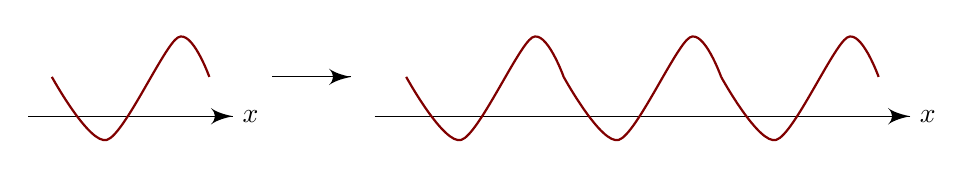
\begin{tikzpicture}
    \draw [->] (-0.3, 0) -- (2.3, 0) node [right] {$x$};
    \draw [mred, thick] plot [smooth] coordinates {(0, 0.5) (0.7, -0.3) (1.6, 1) (2, 0.5)};

    \draw [->] (2.8, 0.5) -- (3.8, 0.5);
    \draw [->] (4.1, 0) -- (10.9, 0) node [right] {$x$};
    \foreach \x in {4.5, 6.5, 8.5} {
      \draw [mred, thick] plot [smooth] coordinates {(\x, 0.5) (\x + 0.7, -0.3) (\x + 1.6, 1) (\x + 2, 0.5)};
    }
  \end{tikzpicture}
\end{center}
So. As mentioned in the previous chapter, we want to find a set of ``basis functions'' for periodic functions. We could go with the simplest case of periodic functions we know of --- the exponential function $e^{in\theta}$. These functions have a period of $2\pi$, and are rather easy to work with. We all know how to integrate and differentiate the exponential function.

More importantly, this set of basis functions is orthogonal. We have
\[
  (e^{im \theta}, e^{in\theta}) = \int_{-\pi}^{\pi} e^{-im\theta} e^{in\theta}\;\d \theta = \int_{-\pi}^\pi e^{i(n - m)\theta}\;\d \theta =
  \begin{cases}
    2\pi & n = m\\
    0    & n\not= m
  \end{cases} = 2\pi \delta_{nm}
\]
We can normalize these to get a set of orthonormal functions $\left\{\frac{1}{\sqrt{2\pi}} e^{in\theta}: n\in \Z\right\}$.

Fourier's idea was to use this as a basis for \emph{any} periodic function. Fourier claimed that any $f: S^1 \to \C$ can be expanded in this basis:
\[
  f(\theta) = \sum_{n \in \Z}\hat{f}_n e^{in\theta},
\]
where
\[
  \hat{f}_n = \frac{1}{2\pi} (e^{in\theta}, f) = \frac{1}{2\pi}\int_{-\pi}^\pi e^{-in\theta} f(\theta)\;\d \theta.
\]
These really should be defined as $f(\theta) = \sum \hat{f}_n \frac{e^{in\theta}}{\sqrt{2\pi}}$ with $\hat{f}_n = \left(\frac{e^{in\theta}}{\sqrt{2\pi}}, f\right)$, but for convenience reasons, we move all the constant factors to the $\hat{f}_n$ coefficients.

We can consider the special case where $f: S^1 \to \R$ is a real function. We might want to make our expansion look a bit more ``real''. We get
\[
  (\hat{f}_n)^* = \left(\frac{1}{2\pi}\int_{-\pi}^\pi e^{-in\theta}f(\theta)\;\d \theta\right)^* = \frac{1}{2\pi}\int_{-\pi}^{\pi}e^{in\theta}f(\theta)\;\d \theta = \hat{f}_{-n}.
\]
So we can replace our Fourier series by
\[
  f(\theta) = \hat{f}_0 + \sum_{n = 1}^\infty\left(\hat{f}_n e^{in\theta} + \hat{f}_{-n}e^{-in\theta}\right) = \hat{f}_0 + \sum_{n = 1}^\infty \left(\hat{f}_n e^{in\theta} + \hat{f}_n^* e^{-in\theta}\right).
\]
Setting $\displaystyle \hat{f}_n = \frac{a_n + ib_n}{2}$, we can write this as
\[
  f(\theta) = \hat{f}_0 + \sum_{n = 1}^\infty (a_n \cos n\theta + b_n \sin n\theta).
\]
Here the coefficients are
\[
  a_n = \frac{1}{\pi}\int_{-\pi}^\pi \cos n\theta f(\theta) \;\d \theta,\quad b_n = \frac{1}{\pi}\int_{-\pi}^\pi \sin n\theta f(\theta) \;\d \theta.
\]
This is an alternative formulation of the Fourier series in terms of $\sin$ and $\cos$.

So when given a real function, which expansion should we use? It depends. If our function is odd (or even), it would be useful to pick the sine/cosine expansion, since the cosine (or sine) terms will simply disappear. On the other hand, if we want to stick our function into a differential equation, exponential functions are usually more helpful.

\subsection{Convergence of Fourier series}
When Fourier first proposed the idea of a Fourier series, people didn't really believe in him. How can we be sure that the infinite series actually converges? It turns out that in many cases, they don't.

To investigate the convergence of the series, we define the \emph{partial Fourier sum} as
\[
  S_n f = \sum_{m = -n}^n \hat{f}_m e^{im\theta}.
\]
The question we want to answer is whether $S_n f$ ``converges'' to $f$. Here we have to be careful with what we mean by convergence. As we (might) have seen in Analysis, there are many ways of defining convergence of functions. If we have a ``norm'' on the space of functions, we can define convergence to mean $\lim\limits_{n\to \infty}\|S_n f - f\| = 0$. Our ``norm'' can be defined as
\[
  \|S_n f - f\| = \frac{1}{2\pi}\int_{-\pi}^\pi |S_n f(\theta) - f(\theta)|^2 \;\d \theta.
\]
However, this doesn't really work if $S_n f$ and $f$ can be arbitrary functions, as in this does not necessarily have to be a norm. Indeed, if $\lim\limits_{n \to \infty}S_n f$ differs from $f$ on finitely or countably many points, the integral will still be zero. In particular, $\lim S_n f$ and $f$ can differ at all rational points, but this definition will say that $S_n f$ converges to $f$.

Hence another possible definition of convergence is to require
\[
  \lim_{n \to \infty}S_n f(\theta) - f(\theta) = 0
\]
for all $\theta$. This is known as \emph{pointwise convergence}. However, this is often too weak a notion. We can ask for more, and require that the \emph{rate} of convergent is independent of $\theta$. This is known as uniform convergence, and is defined by
\[
  \lim_{n \to \infty}\sup_{\theta} |S_n f(\theta) - f(\theta)| = 0.
\]
Of course, with different definitions of convergence, we can get different answers to whether it converges. Unfortunately, even if we manage to get our definition of convergence right, it is still difficult to come up with a criterion to decide if a function has a convergent Fourier Series. As of today, we still don't really understand how the convergence of Fourier series behaves.

Instead of trying to come up with something general, (since this is an applied course), let's look at an example instead.

\begin{eg}
  Consider the sawtooth function $f(\theta) = \theta$.
  \begin{center}
    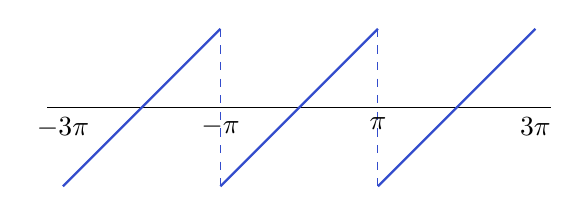
\begin{tikzpicture}
      \draw (-3.2, 0) -- (3.2, 0);

      \draw [thick, mblue] (-3, -1) -- (-1, 1);
      \draw [dashed, mblue] (-1, 1) -- (-1, -1);
      \draw [thick, mblue] (-1, -1) -- (1, 1);
      \draw [dashed, mblue] (1, 1) -- (1, -1);
      \draw [thick, mblue] (1, -1) -- (3, 1);

      \node at (-3, 0) [below] {$-3\pi$};
      \node at (-1, 0) [below] {$-\pi$};
      \node at (1, 0) [below] {$\pi$};
      \node at (3, 0) [below] {$3\pi$};
    \end{tikzpicture}
  \end{center}
  Note that this function is discontinuous at odd multiples of $\pi$.

  The Fourier coefficients (for $n \not= 0$) are
  \[
    \hat{f}_n = \frac{1}{2\pi}\int_{-\pi}^\pi e^{-in\theta}\theta\;\d \theta = \left[-\frac{1}{2\pi i n}e^{-in\theta}\theta\right]_{-\pi}^\pi + \frac{1}{2\pi i n}\int_{-\pi}^\pi e^{in\theta}\;\d \theta = \frac{(-1)^{n + 1}}{in}.
  \]
  We also have $\hat{f}_0 = 0$.

  Hence we have
  \[
    \theta = \sum_{n \not= 0}\frac{(-1)^{n + 1}}{in}e^{in\theta}.
  \]
  It turns out that this series converges to the sawtooth for all $\theta \not= (2m + 1)\pi$, ie. everywhere that the sawtooth is continuous.

  Let's look explicitly at the case where $\theta = \pi$. Each term of the partial Fourier series is zero. So we can say that the Fourier series converges to 0. This is the \emph{average} value of $\lim\limits_{\varepsilon \to 0} f(\pi \pm \varepsilon)$.

  This is typical. At an isolated discontinuity, the Fourier series is the average of the limiting values of the original function. as we approach from either side.
\end{eg}
\subsection{Differentiability and Fourier series}
Integration is a smoothening operator. If we take, say, the step function
\[
  \Theta(x) =
  \begin{cases}
    1 & x > 0\\
    0 & x < 0
  \end{cases}.
\]
Then the integral is given by
\[
  \int \Theta(x)\;\d x =
  \begin{cases}
    x & x > 0\\
    0 & x < 0
  \end{cases}.
\]
This is now a continuous function. If we integrate it again, we make the positive side look like a quadratic curve, and it is now differentiable.
\begin{center}
  \begin{tikzpicture}
    \draw [->] (-2, 0) -- (2, 0) node [right] {$x$};
    \draw [->] (0, -0.5) -- (0, 2.5) node [above] {$y$};
    \draw [mblue, thick] (-2, 0) -- (0, 0);
    \draw [mblue, thick] (0, 2) -- (2, 2);

    \draw [->] (2.5, 1) -- (3.5, 1) node [above, pos=0.5] {$\int\d x$};

    \draw [->] (4, 0) -- (8, 0) node [right] {$x$};
    \draw [->] (6, -0.5) -- (6, 2.5) node [above] {$y$};
    \draw [mred, thick] (4, 0) -- (6, 0);
    \draw [mred, thick] (6, 0) -- (8, 2);
  \end{tikzpicture}
\end{center}
On the other hand, when we differentiate a function, we generally make it worse. For example, when we differentiate the continuous function $\int \Theta (x)\;\d x$, we obtain the discontinuous function $\Theta(x)$. If we attempt to differentiate this again, we get the $\delta$-(non)-function.

Hence, it is often helpful to characterize the ``smoothness'' of a function by how many times we can differentiate it. It turns out this is rather relevant to the behaviour of the Fourier series.

Suppose that we have a function that is itself continuous and whose first $m - 1$ derivatives are also continuous, but $f^{(m)}$ has isolated discontinuities at $\{\theta_1, \theta_2, \theta_3, \cdots, \theta_r\}$.

We can look at the $k$th Fourier coefficient:
\begin{align*}
  \hat{f}_k &= \frac{1}{2\pi}\int_{-\pi}^\pi e^{-k\theta}f(\theta) \;\d \theta\\
  &= \left[-\frac{1}{2\pi i k}e^{-ik\theta}f(\theta)\right]^{\pi}_{-\pi} + \frac{1}{2\pi i k}\int_{-\pi}^\pi e^{-ik\theta}f'(\theta)\;\d \theta\\
  \intertext{The first term vanishes since $f(\theta)$ is continuous and takes the same value at $\pi$ and $-\pi$. So we are left with}
  &= \frac{1}{2\pi i k}\int_{-\pi}^\pi e^{-ik\theta}f'(\theta)\;\d \theta\\
  &= \cdots\\
  &= \frac{1}{(ik)^m}\frac{1}{2\pi} \int_{-\pi}^\pi e^{ik\theta} f^{(m)}(\theta)\;\d \theta.
  \intertext{Now we have to be careful, since $f^{(m)}$ is no longer continuous. However provided that $f^{(m)}$ is everywhere finite, we can approximate this by removing small strips $(\theta_i - \varepsilon, \theta_i + \varepsilon)$ from our domain of integration, and take the limit $\varepsilon \to 0$. We can write this as}
  &= \lim_{\varepsilon \to 0}\frac{1}{(ik)^m}\frac{1}{2\pi}\int_{-\pi}^{\theta_1 - \varepsilon} + \int_{\theta_1 + \varepsilon}^{\theta_2 - \varepsilon} + \cdots + \int_{\theta_r + \varepsilon}^{\pi} e^{ik\theta} f^{(m)}(\theta)\;\d \theta\\
  &= \frac{1}{(ik)^{m + 1}} \frac{1}{2\pi}\left[\sum_{s = 1}^r (f^{(m)}(\theta_s^+) - f^{(m)}(\theta_s^-)) + \int_{(-\pi, \pi)\setminus \theta} e^{-ik\theta} f^{(m + 1)}(\theta) \;\d \theta\right].
\end{align*}
We now have to stop. So $\hat{f}_k$ decays like $\left(\frac{1}{k}\right)^{m + 1}$ if our function and its $(m - 1)$ derivatives are continuous. This means that if a function is more differentiable, then the coefficients decay more quickly.

This makes sense. If we have a rather smooth function, then we would expect the first few Fourier terms (with low frequency) to account for most of the variation of $f$. Hence the coefficients decay really quickly.

However, if the function is jiggly and bumps around all the time, we would expect to need some higher frequency to account for the minute variation. Hence the terms would not decay away that quickly. Hence if we can differentiate it more times, then in general the terms should decay quicker.

\begin{thm}[Parseval's theorem]
  \[
    (f, f) = \int_{-\pi}^\pi |f(\theta)|^2 \;\d \theta = 2\pi \sum_{n\in \Z}|\hat{f}_n|^2
  \]
\end{thm}

\begin{proof}
  \begin{align*}
    (f, f) &= \int_{-\pi}^\pi |f(\theta)|^2 \;\d \theta\\
    &= \int_{-\pi}^{\pi} \left(\sum_{m \in \Z} \hat{f}_m^* e^{-im\theta}\right)\left(\sum_{n \in \Z} \hat{f}_n e^{in\theta}\right)\;\d \theta\\
    &= \sum_{m, n\in \Z}\hat{f}_m^* \hat{f}_n \int_{-\pi}^\pi e^{i(n - m)\theta}\;\d \theta\\
    &= 2\pi \sum_{m, n\in \Z}\hat{f}_m^* \hat{f}_n \delta_{mn}\\
    &= 2\pi \sum_{n\in \Z}|\hat{f}_n|^2
  \end{align*}
\end{proof}
Note that this is not a fully rigorous proof, since we assumed not only that the Fourier series converges to the function, but also that we could commute the infinite sums. However, for the purposes of an applied course, this is sufficient.

Last time, we computed that the sawtooth function $f(\theta) = \theta$ has Fourier coefficients
\[
  \hat{f}_0 = 0,\quad \hat{f}_n = \frac{i(-1)^{n}}{n}\text{ for }n\not= 0.
\]
But why do we care? It turns out this has some applications in number theory. You might have heard of the Riemann $\zeta$-function, defined by
\[
  \zeta(s) = \sum_{n = 1}^\infty \frac{1}{n^s}.
\]
We will show that this obeys the property that for any $m$, $\zeta(2m) = \pi^{2m}q$ for some $q\in \Q$. This may not be obvious at first sight. So let's apply Parseval's theorem for the sawtooth. By direct computation, we know that
\[
  (f, f) = \int_{-\pi}^\pi \theta^2 \;\d \theta = \frac{2\pi^3}{3}.
\]
However, by Parseval's theorem, we know that
\[
  (f, f) = 2\pi \sum_{n \in \Z}|\hat{f}_n|^2 = 4\pi \sum_{n = 1}^\infty \frac{1}{n^2}.
\]
Putting these together, we learn that
\[
  \sum_{n = 1}^\infty \frac{1}{n^2} = \zeta(2) = \frac{\pi^2}{6}.
\]
We have just done it for the case where $m = 1$. But if we integrate the sawtooth function repeatedly, then we can get the general result for all $m$.

At this point, we might ask, why are we choosing these $e^{im\theta}$ as our basis? Surely there are a lot of different sets of basis we can use. For example, infinite dimensions, we can just arbitrary choose random vectors (that are not linearly dependent) to get a set of basis vectors. However, in practice, we don't pick them randomly. We often choose a basis that can reveal the symmetry of a system. For example, if we have a rotationally symmetric system, we would like to use polar coordinates. Similarly, if we have periodic functions, then $e^{im\theta}$ is often a good choice of basis.

\section{Sturm-Liouville Theory}
In finite dimensions, we often consider \emph{linear maps} $M: V\to W$. If $\{\mathbf{v}_i\}$ is a basis for $V$ and $\{\mathbf{w}\}$ is a basis for $W$, then we can represent the map by a matrix with entries
\[
  M_{ai} = (\mathbf{w}_a, M\mathbf{v}_i).
\]
A map $M: V\to V$ is called \emph{self-adjoint} if $M^\dagger = M$ as matrices. However, it is not obvious how we can extend this notion to arbitrary maps between arbitrary vector spaces (with an inner product) when they cannot be represented by a matrix.

Instead, we can define the \emph{adjoint} $B$ of a map $A: V\to V$ to be a map such that
\[
  (B\mathbf{u}, \mathbf{v}) = (\mathbf{u}, A\mathbf{v})
\]
for all vectors $\mathbf{u}, \mathbf{v}\in V$. A map is then self-adjoint if
\[
  (M\mathbf{u}, \mathbf{v}) = (\mathbf{u}, M\mathbf{v}).
\]
Self-adjoint matrices come with a natural basis. Recall that the \emph{eigenvalues} of a matrix are the roots of $\det(M - \lambda I) = 0$. The \emph{eigenvector} corresponding to an eigenvalue $\lambda$ is defined by $M\mathbf{v}_i = \lambda_i \mathbf{v}_i$.

In general, eigenvalues can be any complex number. However, self-adjoint maps have \emph{real} eigenvalues. Suppose
\[
  M\mathbf{v}_i = \lambda_i \mathbf{v}_i.
\]
Then we have
\[
  \lambda_i (\mathbf{v}_i, \mathbf{v}_i) = (\mathbf{v}_i, M\mathbf{v}_i) = (M\mathbf{v}_i, \mathbf{v}_i) = \lambda_i^* (\mathbf{v}_i, \mathbf{v}_i).
\]
So $\lambda_i = \lambda_i^*$.

Furthermore, eigenvectors with distinct eigenvalues are orthogonal with respect to the inner product. Suppose that
\[
  M \mathbf{v}_i = \lambda_i \mathbf{v}_i,\quad M \mathbf{v}_j = \lambda_j \mathbf{v}_j.
\]
Then
\[
  \lambda_i (\mathbf{v}_j, \mathbf{v}_i) = (\mathbf{v}_j, M\mathbf{v}_i) = (M\mathbf{v}_j, \mathbf{v}_i) = \lambda_j(\mathbf{v}_j, \mathbf{v}_i).
\]
Since $\lambda_i \not= \lambda_j$, we must have $(\mathbf{v}_j, \mathbf{v}_i) = 0$.

Knowing eigenvalues and eigenvalues gives a neat way so solve linear equations of the form
\[
  M \mathbf{u} = \mathbf{f}.
\]
Here we are given $M$ and $\mathbf{f}$, and want to find $\mathbf{u}$. Of course, the answer is $\mathbf{u} = M^{-1}f$. However, if we expand in terms of eigenvectors, we obtain
\[
  M\mathbf{u} = M\sum u_i \mathbf{v}_i = \sum u_i \lambda_i \mathbf{v}_i.
\]
Hence we have
\[
  \sum u_i \lambda_i \mathbf{v}_i = \sum f_i \mathbf{v}_i.
\]
Taking the inner product with $\mathbf{v}_j$, we know that
\[
  u_j = \frac{f_j}{\lambda_j}.
\]
So far, these are all things from IA Vectors and Matrices. Sturm-Liouville theory is the infinite-dimensional analogue.

In our vector space of differentiable functions, our ``matrices'' would be linear differential operators $\mathcal{L}$. For example, we could have
\[
  \mathcal{L} = A_p(x) \frac{\d^p}{\d x^p} + A_{p - 1}(x) \frac{\d^{p - 1}}{\d x^{p - 1}} + \cdots + A_1(x)\frac{\d}{\d x} + A_0(x).
\]
It is an easy check that this is in fact linear.

We say $\mathcal{L}$ has order $p$ if the highest derivative that appears is $\frac{\d^p}{\d x^p}$.

In most applications, we will be interested in the case $p = 2$. When will our $\mathcal{L}$ be self-adjoint?

In the $p = 2$ case, we have
\begin{align*}
  \mathcal{L} y &= P \frac{\d^2 y}{\d x^2} + R \frac{\d y}{\d x} - Q y \\
  &= P\left[\frac{\d^2 y}{\d x^2} + \frac{R}{P}\frac{\d y}{\d x} - \frac{Q}{P}y\right] \\
  &= P\left[e^{-\int \frac{R}{P}\;\d x}\frac{\d}{\d x}\left(e^{\int \frac{R}{P}\;\d x}\frac{\d y}{\d x}\right)- \frac{Q}{P}y\right]\\
  \intertext{Let $p = \exp\left(\int \frac{R}{P}\;\d x\right)$. Then we can write this as}
  &= P p^{-1}\left[\frac{\d}{\d x}\left(p\frac{\d y}{\d x}\right) - \frac{Q}{P}p y\right].
\end{align*}
We further define $q = \frac{Q}{P}p$. We also drop a factor of $Pp^{-1}$. Then we are left with
\[
  \mathcal{L} = \frac{\d}{\d x}\left(p(x)\frac{\d}{\d x}\right) - q(x).
\]
This is the \emph{Sturm-Liouville form} of the operator. Now let's compute $(f, \mathcal{L}g)$. We integrate by parts numerous times to obtain
\begin{align*}
  (f, \mathcal{L}g) &= \int_a^b f^*\left(\frac{\d}{\d x}\left(p \frac{\d g}{\d x}\right) - qg\right)\;\d x \\
  &= [f^* pg']_a^b - \int_a^b \left(\frac{\d f^*}{\d x}p\frac{\d g}{\d x} + f^* qg\right)\;\d x\\
  &= [f^*pg' - f'^*pg]_a^b + \int_a^b \left(\frac{\d}{\d x}\left(p\frac{\d f^*}{\d x}\right) - qf^*\right)g\;\d x\\
  &= [(f^*g' - f'^*g)p]_a^b + (\mathcal{L}f, g),
\end{align*}
assuming that $p, q$ are real.

So 2nd order linear differential operators are self-adjoint with respect to this norm if $p, q$ are real and the boundary terms vanish. When do the boundary terms vanish? One possibility is when $p$ is periodic (with the right period), or if we constrain $f$ and $g$ to be periodic.

\begin{eg}
  We can consider a simple case, where
  \[
    \mathcal{L} = \frac{\d^2}{\d x^2}.
  \]
  Here we have $p = 1, q = 0$. If we ask for functions to be periodic on $[a, b]$, then
  \[
    \int_a^b f^*\frac{\d^2 g}{\d x^2}\;\d x = \int_a^b \frac{\d^2 f^*}{\d x^2}g\;\d x.
  \]
  Note that it is important that we have a \emph{second-order} differential operator. If it is first-order, then we would have a negative sign, since we integrated by parts once.
\end{eg}

Just as in finite dimensions, self-adjoint operators have eigenfunctions and eigenvalues with special properties. First, we define a more sophisticated inner product.
\begin{defi}[Inner product with weight]
  An \emph{inner product with weight} $w$, written $(\ph, \ph)_w$, is defined by
  \[
    (f, g)_w = \int_a^b f^*(x) g(x) w(x)\;\d x,
  \]
  where $w$ is real, non-negative, and has only finitely many zeroes.
\end{defi}
Why do we want a weight $w(x)$? In the future, we might want to work with the unit disk, instead of a square in $\R^2$. When we want to use polar coordinates, we will have to integrate with $r\;\d r\;\d \theta$, instead of just $\d r\;\d \theta$. Hence we need the weight of $r$. Also, we allow it to have finitely many zeroes, so that the radius can be $0$ at the origin.

Why can't we have more zeroes? We want the inner product to keep the property that $(f, f)_w = 0$ iff $f = 0$ (for continuous $f$). If $w$ is zero at too many places, then the inner product could be zero without $f$ being zero.

We now define what it means to be an eigenfuction.
\begin{defi}[Eigenfunction with weight]
  An \emph{eigenfunction with weight} $w$ of $\mathcal{L}$ is a function $y: [a, b] \to \C$ obeying the differential equation
  \[
    \mathcal{L} y = \lambda w y,
  \]
  where $\lambda\in \C$ is the eigenvalue.
\end{defi}
This might be strange at first sight. It seems like we can take any nonsense $y$, apply $\mathcal{L}$, to get some nonsense $\mathcal{L} y$. But then it is fine, since we can write it as some nonsense $w$ times our original $y$. So any function is an eigenfunction? No! There are many constraints $w$ has to satisfy, like being positive, real and having finitely many zeroes. It turns out this severely restraints what values $y$ can take, so not everything will be an eigenfunction. In fact we can develop this theory without the weight function $w$. However, weight functions are much more convenient when, say, dealing with the unit disk.

\begin{prop}
  The eigenvalues of a Sturm-Liouville operator are real.
\end{prop}

\begin{proof}
  Suppose $\mathcal{L} y_i = \lambda_i w y_i$. Then
  \[
    \lambda_i (y_i, y_i)_w = \lambda_i (y_i, w y_i) = (y_i, \mathcal{L} y_i) = (\mathcal{L} y_i, y_i) = (\lambda_i w y_i, y_i) = \lambda_i^* (y_i, y_i)_w.
  \]
  Since $(y_i, y_i)_w \not= 0$, we have $\lambda_i = \lambda_i^*$.
\end{proof}
Note that the first and last terms use the weighted inner product, but the middle terms use the unweighted inner product.

\begin{prop}
  Eigenfunctions with different eigenvalues (but same weight) are orthogonal.
\end{prop}

\begin{proof}
  Let $\mathcal{L} y_i = \lambda_i w y_i$ and $\mathcal{L} y_j = \lambda_j w y_j$. Then
  \[
    \lambda_i (y_j, y_i)_w = (y_j, \mathcal{L} y_i) = (\mathcal{L} y_j, y_i) = \lambda_j (y_j, y_i)_w.
  \]
  Since $\lambda_i \not= \lambda_j$, we must have $(y_j, y_i)_w = 0$.
\end{proof}

\begin{prop}
  On a \emph{compact} domain, the eigenvalues $\lambda_1, \lambda_2, \cdots$ form a countably infinite sequence and are discrete.
\end{prop}
We will not prove this.

This will be a rather helpful result in quantum mechanics, since in quantum mechanics, the possible values of, say, the energy are the eigenvalues of the Hamiltonian operator. Then this result says that the possible values of the energy are discrete and form an infinite sequence.

Note here the word \emph{compact}. In quantum mechanics, if we restrict a particle in a well $[0, 1]$, then it will have quantized energy level since the domain is compact. However, if the particle is free, then it can have any energy at all since we no longer have a compact domain. Similarly, angular momentum is quantized, since it describe rotations, which takes values in $S^1$, which is compact.

\begin{prop}
  The eigenfunctions are complete: any function $f: [a, b] \to \C$ (obeying appropriate boundary conditions) can be expanded as
  \[
    f(x) = \sum_n \hat{f}_n y_n(x),
  \]
  where
  \[
    \hat{f}_n = \int y^*_n(x) f(x) w(x)\;\d x.
  \]
\end{prop}

\begin{eg}
  Let $[a, b] = [-L, L]$, $\mathcal{L} = \frac{\d^2}{\d x^2}$, $w = 1$, restricting to periodic functions Then our eigenfunction obeys
  \[
    \frac{\d^2 y_n}{\d x^2} = \lambda_n y_n(x),
  \]
  Then our periodic functions are
  \[
    y_n(x) = \exp\left(\frac{in\pi x}{L}\right)
  \]
  with eigenvalues
  \[
    \lambda_n = - \frac{n^2 \pi^2}{L^2}
  \]
  for $n \in \Z$. This is just the Fourier series!
\end{eg}

\begin{eg}[Hermite polynomials]
  We are going to cheat a little bit and pick our domain to be $\R$. We want to study the differential equation
  \[
    \frac{1}{2}H'' - xH' = \lambda H,
  \]
  with $H: \R \to \C$. We want to put this in Sturm-Liouville form. We have
  \[
    p(x) = \exp\left(-\int_0^x 2t \;\d t\right) = e^{-x^2},
  \]
  ignoring constant factors. Then $q(x) = 0$. We can rewrite this as
  \[
    \frac{\d}{\d x}\left(e^{-x^2}\frac{\d H}{\d x}\right) = -2\lambda e^{-x^2} H(x).
  \]
  So we take our weight function to be $w(x) = e^{-x^2}$.

  We now ask that $H(x)$ grows at most polynomially as $|x| \to \infty$. In particular, we want $e^{-x^2}H(x)^2 \to 0$. This ensures that the boundary terms from integration by parts vanish at the infinite boundary, so that our Sturm-Liouville operator is self-adjoint.

  The eigenfunctions turn out to be
  \[
    H_n(x) = (-1)^n e^{x^2}\frac{\d^n}{\d x^n}\left(e^{-x^2}\right).
  \]
  These are known as the \emph{Hermite polynomials}. Note that these are indeed polynomials. When we differentiate the $e^{-x^2}$ term many times, we get a lot of things from the product rule, but they will always keep an $e^{-x^2}$, which will ultimately cancel with $e^{x^2}$.
\end{eg}

Just as for matrices, we can use the eigenfunction expansion to solve forced differential equations. For example, if might want to solve
\[
  \mathcal{L} g = f(x),
\]
where $f(x)$ is a forcing term. We can write this as
\[
  \mathcal{L} g = w(x) F(x).
\]
We exapnd our $g$ as
\[
  g(x) = \sum_{n \in \Z}\hat{g}_n y_n(x).
\]
Then by linearity,
\[
  \mathcal{L}g = \sum_{n \in \Z}\hat{g}_n \mathcal{L} y_n(x) = \sum_{n \in \Z}\hat{g}_n \lambda_n w(x)y_n(x).
\]
We can also expand our forcing function as
\[
  w(x) F(x) = w(x) \left(\sum_{n \in \Z}\hat{F}_n y_n(x)\right).
\]
Taking the (regular) inner product with $y_m(x)$ (and noting orthogonality of eigenfunctions), we obtain
\[
  w(x) \hat{g}_m \lambda_m = w(x) \hat{F}_m
\]
This tells us that
\[
  \hat{g}_m = \frac{\hat{F}_m}{\lambda_m}.
\]
So we have
\[
  g(x) = \sum_{n \in \Z}\frac{\hat{F}_n}{\lambda_n}y_n(x),
\]
provided all $\lambda_n$ are non-zero.

This is a systematic way of solving forced differential equations. We used to solve these by ``being smart''. We just looked at the forcing term and tried to guess what would work. Unsurprisingly, this approach does not suceed all the time. Thus it is helpful to have a systematic way of solving the equations.

It is often helpful to rewrite this into another form, using the fact that $\hat{F}_n = (y_n, F)_w$. So we have
\[
  g(x) = \sum_{n \in \Z}\frac{1}{\lambda_n}(y_n, F)_w y_n(x) = \int_a^b \sum_{n \in \Z}\frac{1}{\lambda_n} y_n^*(t) y_n(x) w(t) F(t)\;\d t.
\]
Note that we swapped the sum and the integral, which is in general a dangerous thing to do, but we don't really care because this is an applied course. We can further write the above as
\[
  g(x) = \int_a^b G(x, t) F(t) w(t)\;\d t,
\]
where $G(x, t)$ is the infinite sum
\[
  G(x, t) = \sum_{n \in \Z}\frac{1}{\lambda_n}y_n^*(t) y_n(x).
\]
Note that this depends on $\lambda_n$ and $y_n$ only. It depends on the differential operator $\mathcal{L}$, but not the forcing term $F$. We can think of this as something like the ``inverse matrix'', which we can use to solve the forced differential equation for any forcing term.

Recall that for a matrix, the inverse exists if the determinant is non-zero, which is true if the eigenvalues are all non-zero. Similarly, here a necessary condition for the Green's function to exist is that all the eigenvalues are non-zero.

We now have a second version of Perseval's theorem.
\begin{thm}[Perseval's theorem II]
  \[
    (f, f)_w = \sum_{n \in \Z}|\hat{f}_n|^2.
  \]
\end{thm}

\begin{proof}
  We have
  \begin{align*}
    (f, f)_w &= \int_\Omega f^*(x) f(x) w(x) \;\d x\\
    &= \sum_{n, m \in \Z}\int_\Omega \hat{f}^*_n y_n^*(x) \hat{f}_m y_m(x)w(x)\;\d x\\
    &= \sum_{n, m\in \Z}\hat{f}^*_n \hat{f}_m (y_n, y_m)_w  \\
    &= \sum_{n \in \Z}|\hat{f}_n|^2.
  \end{align*}
\end{proof}

\subsection{Least squares approximation}
So far, we have expanded functions in terms of infinite series. However, in real life, when we ask a computer to do this for us, it is incapable of storing and calculating an infinite series. So we need to truncate it at some point.

Suppose we approximate some function $f: \Omega \to \C$ by a \emph{finite} set of eigenfunctions $y_n(x)$. Suppose we write the approximation $g$ as
\[
  g(x) = \sum_{k = 1}^n c_k y_k(x).
\]
The objective here is to figure out what values of the coefficients $c_k$ are ``the best'', ie. can make $g$ represent $f$ as closely as possible.

Firstly, we have to make it explicit what we mean by ``as closely as possible''. Here we take this to mean that we want to minimize the $w$-norm $(f - g, f - g)_w$. By linearity of the norm, we know that
\[
  (f - g, f - g)_w = (f, f)_w + (g, g)_w - (f, g)_w - (g, f)_w.
\]
To minimize this norm, we want
\[
  0 = \frac{\partial}{\partial c_j} (f - g, f - g)_w = \frac{\partial}{\partial c_j}[(f, f)_w + (g, g)_w - (f, g)_w - (g, f)_w].
\]
We know that the $(f, f)_w$ term vanishes since it does not depend on $c_k$. Expanding our definitions of $g$, we can get
\[
  0 = \frac{\partial}{\partial c_j}\left(\sum_{i = 1}^\infty |c_k|^n - \sum_{k = 1}^n \hat{f}_k^* c_k  - \sum_{k = 1}^n c_k^* \hat{f}_k\right) = c^*_j - \hat{f}_j^*.
\]
Note that here we are treating $c_j^*$ and $c_j$ as distinct quantities. So when we vary $c_j$, $c_j^*$ is unchanged. To formally justify this treatment, we can vary the real and imaginary parts separately.

Hence, the extremum is achieved at $c_j^* = \hat{f}_j^*$. Similarly, varying with respect to $c_j^*$, we get that $c_j = \hat{f}_j$.

To check that this is indeed an minimum, we can look at the second-derivatives
\[
  \frac{\partial^2}{\partial c_i \partial c_j} (f - g, f - g)_w = \frac{\partial^2}{\partial c_i^* c_j^*} (f - g, f - g)_w = 0,
\]
while
\[
  \frac{\partial^2}{\partial c_i^* \partial c_j} (f - g, f - g)_w = \delta_{ij} \geq 0.
\]
Hence this is indeed a minimum.

Thus we know that $(f - g, f - g)_w$ is minimized over all $g(x)$ when
\[
  c_k = \hat{f}_k = (y_k, f)_w.
\]
These are exactly the coefficients in our infinite expansion. Hence if we truncate our series at an arbitrary point, it is still the best approximation we can get.

\section{Partial differential equations}
So far, we have come up with a lot of general theory about functions and stuff. We are going to look into some applications of these.
\subsection{Laplace's equation}
\begin{defi}[Laplace's equation]
  \emph{Laplace's equation} on $\R^n$ says that a (twice-differentiable) equation $\phi: \R^n \to \C$ obeys
  \[
    \nabla^2 \phi = 0,
  \]
  where
  \[
    \nabla^2 = \sum_{i = 1}^n \frac{\partial^2}{\partial x_i^2}.
  \]
\end{defi}
This equation arises in many situations. For example, if we have a conservative force $\mathbf{F} = -\nabla \phi$, and we are in a region where the force obeys the source-free Gauss' law $\nabla\cdot \mathbf{F} = 0$ (eg. when there is no electric charge in an electromagnetic field), then we get Laplace's equation.

It also arises as a special case of the heat equation $\frac{\partial \phi}{\partial t} = \kappa \nabla^2 \phi$, and wave equation $\frac{\partial^2 \phi}{\partial t^2} = c^2 \nabla^2 \phi$, when there is no time dependence.

\begin{defi}[Harmonic functions]
  Functions that obey Laplace's equation are often called \emph{harmonic functions}.
\end{defi}

\begin{prop}
  Let $\Omega$ be a compact domain, and $\nabla \Omega$ be its boundary. Let $ f: \partial \Omega\to \R$. Then there is a unique solution to $\nabla^2 \phi = 0$ on $\Omega$ with $\phi|_{\partial \Omega} = f$.
\end{prop}

\begin{proof}
  Suppose $\phi_1$ and $\phi_2$ are both solutions such that $\phi_1|_{\partial \Omega} = \phi_2|_{\partial \Omega} = f$. Then let $\Phi = \phi_1 - \phi_2$. So $\Phi = 0$ on the boundary. So we have
  \[
    0 = \int_\Omega \Phi \nabla^2 \Phi \;\d^n x  = -\int_\Omega (\nabla \Phi) \cdot (\nabla \Phi)\;\d x + \int_{\partial \Omega} \Phi \nabla \Phi\cdot \mathbf{n} \;\d^{n -1 }x.
  \]
  We note that the second term vanishes since $\Phi = 0$ on the boundary. So we have
  \[
    0 = -\int_\Omega (\nabla \Phi) \cdot (\nabla \Phi)\;\d x.
  \]
  However, we know that $(\nabla \Phi) \cdot (\nabla \Phi) \geq 0$ with equality iff $\nabla \Phi = 0$.  Hence $\Phi$ is constant throughout $\Omega$. Since at the boundary, $\Phi = 0$, we have $\Phi = 0$ throughout, ie. $\phi_1 = \phi_2$.
\end{proof}

Asking that $\phi|_{\partial \Omega} = f(x)$ is a \emph{Dirichlet} boundary condition. We can instead ask $\mathbf{n}\cdot \nabla \phi|_{\partial \Omega} = g$, a Neumann condition. In this case, we have a unique solution up to a constant factor.

These we've all seen in IA Vector Calculus, but this time in arbitrary dimensions.

\subsection{Laplace's equation in the unit disk in \texorpdfstring{$\R^2$}{R2}}
Let $\Omega = \{(x, y) \in \R^2: x^2 + y^2 \leq 1\}$.  Then Laplace's equation becomes
\[
  0 = \nabla^2 \phi = \frac{\partial^2 \phi}{\partial x^2} + \frac{\partial^2 \phi}{\partial y^2} = \frac{\partial^2 \phi}{\partial z \partial \bar{z}},
\]
where we define $z = x + iy, \bar z = x - iy$. Then the general solution is
\[
  \phi(z, \bar z) = \psi(z) + \chi(\bar z)
\]
for some $\psi, \chi$.

Suppose we want a solution obeying the Dirichlet boundary condition $\phi(z, \bar z) |_{\partial \Omega} = f(\theta)$, where the boundary $\partial \Omega$ is the unit circle. Since the domain is the unit circle $S^1$, we can Fourier-expand it! We can write
\[
  f(\theta) = \sum_{n \in \Z}\hat{f}_n e^{in\theta} = \hat{f}_0 + \sum_{n = 1}^\infty \hat{f}_n e^{in\theta} + \sum_{n = 1}^\infty \hat{f}_{-n} e^{-in\theta}.
\]
However, we know that $z = re^{i\theta}$ and $\bar{z} = re^{i\theta}$. So on the boundary, we know that $z = e^{i\theta}$ and $\bar z = e^{-i\theta}$. So we can write
\[
  f(\theta) = \hat{f}_0 + \sum_{n = 1}^\infty (\hat{f}_n z^n + \hat{f}_{-n}\bar{z}^n)
\]
This is defined for $|z| = 1$. Now we can define $\phi$ on the unit disk by
\[
  \phi(z, \bar z) = \hat{f}_0 + \sum_{n = 1}^\infty \hat{f}_n z^n + \sum_{n = 1}^\infty \hat{f}_{-n}\bar{z}^n.
\]
It is clear that this obeys the boundary conditions by construction. Also, $\phi(z, \bar{z})$ certainly converges when $|z| < 1$ if the series for $f(\theta)$ converged on $\partial \Omega$. Also, $\phi(z, \bar z)$ is of the form $\psi(z) + \chi(\bar z)$. So it is a solution to Laplace's equation on the unit disk. Since the solution is unique, we're done!

\subsection{Separation of variables}
Unfortunately, the use of complex variables is very special to the case where $\Omega \subseteq \R^2$. In higher dimensions, we proceed differently.

We let $\Omega = \{(x, y, z) \in \R^3: 0 \leq x \leq a, 0 \leq y \leq b, z \geq 0\}$. We want the following boundary conditions:
\begin{align*}
  \psi(0, y, z) &= \psi(a, y, z) = 0\\
  \psi(x, 0, z) &= \psi(x, b, z) = 0\\
  \lim_{z\to \infty} \psi(x, y, z) &= 0\\
  \psi(x, y, 0) &= f(x, y),
\end{align*}
where $f$ is a given function. In other words, we want our function to be $f$ when $z = 0$ and vanish at the boundaries.

The first step is to look for a solution of $\nabla^2 \psi(x, y, z) = 0$ of the form
\[
  \psi(x, y, z) = X(x)Y(y)Z(z).
\]
Then we have
\[
  0 = \nabla^2 \psi = YZX'' + XZY'' + XYZ'' = XYZ \left(\frac{X''}{X} + \frac{Y''}{Y} + \frac{Z''}{Z}\right).
\]
As long as $\psi \not= 0$, we can divide through by $\psi$ and obtain
\[
  \frac{X''}{X} + \frac{Y''}{Y} + \frac{Z''}{Z} = 0.
\]
The key point is each term depends on only \emph{one} of the variables $(x, y, z)$. If we vary, say, $x$, then $\frac{Y''}{Y} + \frac{Z''}{Z}$ does not change. For the total sum to be $0$, $\frac{X''}{X}$ must be constant. So each term has to be separately constant. We can thus write
\[
  X'' = -\lambda X,\quad Y'' = -\mu Y,\quad Z'' = (\lambda + \mu) Z.
\]
The signs before $\lambda$ and $\mu$ are there just to make our life easier later on.

We can solve these to obtain
\begin{align*}
  X &= a\sin \sqrt{\lambda} x + b \cos \sqrt{\lambda} x,\\
  Y &= c\sin \sqrt{\lambda} y + d \cos \sqrt{\lambda} x,\\
  Z &= g\exp(\sqrt{\lambda + \mu} z) + h\exp(-\sqrt{\lambda + \mu} z).
\end{align*}
We now impose the homogeneous boundary conditions, ie. the conditions that $\psi$ vanishes at the walls and at infinity.
\begin{itemize}
  \item At $x = 0$, we need $\psi(0, y, z) = 0$. So $b = 0$.
  \item At $x = a$, we need $\psi(a, y, z) = 0$. So $\lambda = \left(\frac{n\pi}{a}\right)^2$.
  \item At $y = 0$, we need $\psi(x, 0, z) = 0$. So $d = 0$.
  \item At $y = b$, we need $\psi(x, b, z) = 0$. So $\mu = \left(\frac{m\pi}{b}\right)^2$.
  \item As $z \to \infty$, $\psi(x, y, z) \to 0$. So $g = 0$.
\end{itemize}
Here we have $n, m \in \N$.

So we found a solution
\[
  \psi(x, y, z) = A_{n, m}\sin \left(\frac{n\pi x}{a}\right) \sin \left(\frac{m\pi y}{b}\right) \exp(-s_{n, m} z),
\]
where $A_{n, m}$ is an arbitrary constant, and
\[
  s_{n, m}^2 = \left(\frac{n^2}{a^2} + \frac{m^2}{b^2}\right)\pi^2.
\]
This obeys the homogeneous boundary conditions for any $n, m \in \N$ but not the inhomogeneous condition at $z = 0$.

By linearity, the general solution obeying the homogeneous boundary conditions is
\[
  \psi(x, y, z) = \sum_{n, m = 1}^{\infty} A_{n, m} \sin\left(\frac{n\pi x}{a}\right) \sin \left(\frac{m\pi y}{b}\right) \exp(-s_{n, m} z)
\]
The final step is to impose the inhomogeneous boundary condition $\psi(x, y, 0) = f(x, y)$. In other words, we need
\[
  \sum_{n, m = 1}^{\infty} A_{n, m} \sin\left(\frac{n\pi x}{a}\right) \sin \left(\frac{m\pi y}{b}\right)  = f(x, y). \tag{$\dagger$}
\]
The objective is thus to find the $A_{n, m}$ coefficients.

We can use the orthogonality relation we've previously had:
\[
  \int_0^a \sin\left(\frac{k\pi x}{a}\right) \sin \left(\frac{n\pi x}{a}\right)\;\d x = \delta_{k, n} \frac{a}{2}.
\]
So we multiply $(\dagger)$ by $\sin \left(\frac{k\pi x}{a}\right)$ and integrate:
\[
  \sum_{n, m = 1}^\infty A_{n, m}\int_0^a \sin \left(\frac{k\pi x}{a}\right) \sin \left(\frac{n\pi x}{a}\right)\;\d x \sin\left(\frac{m\pi y}{b}\right) = \int_0^a \sin\left(\frac{k \pi x}{a}\right)f(x, y) \;\d x.
\]
Using the orthogonality relation, we have
\[
  \frac{a}{2}\sum_{m = 1}^\infty A_{k, m} \sin\left(\frac{m\pi y}{b}\right) = \int_0^a \sin\left(\frac{k\pi x}{a}\right) f(x, y)\;\d x.
\]
We can perform the same trick again, and obtain
\[
  \frac{ab}{4}A_{k, j} = \int_{[0, a]\times [0, b]}\sin \left(\frac{k\pi x}{a}\right) \sin\left(\frac{j\pi y}{b}\right) f(x, y)\;\d x\;\d y.\tag{$*$}
\]
So we found the solution
\[
  \psi(x, y, z) = \sum_{n, m = 1}^{\infty} A_{n, m} \sin\left(\frac{n\pi x}{a}\right) \sin \left(\frac{m\pi y}{b}\right) \exp(-s_{n, m} z)
\]
where $A_{m, n}$ is given by $(*)$.  Since we have shown that there is a unique solution to Laplace's equation obeying Dirichlet boundary conditions, we're done.

Note that if we imposed a boundary condition at finite $z$, say $0 \leq z \leq c$, then both sets of exponential $\exp (\pm \sqrt{\lambda + \mu} z)$ would have contributed. Similarly, if $\psi$ does not vanish at the other boundaries, then the $\cos$ terms would also contribute.

In general, to actually find our $\psi$, we have to do the horrible integral for $A_{m, n}$, and this is not always easy (since integrals are \emph{hard}). We will just look at a simple example.
\begin{eg}
  Suppose $f(x, y) = 1$. Then
  \[
    A_{m, n} = \frac{4}{ab} \int_0^a \sin \left(\frac{n\pi x}{a}\right)\;\d x \int_0^ b \sin \left(\frac{m\pi y}{b}\right)\;\d y =
    \begin{cases}
      \frac{16}{\pi^2 mn} & n, m\text{ both odd}\\
      0 & \text{otherwise}
    \end{cases}
  \]
  Hence we have
  \[
    \psi(x, y, z) = \frac{16}{\pi^2}\sum_{n, m\text{ odd}} \frac{1}{nm}\sin\left(\frac{n\pi x}{a}\right) \sin \left(\frac{m\pi y}{b}\right) \exp(-s_{m, n}z).
  \]
\end{eg}

\subsection{Laplace's equation in spherical polar coordinates}
\subsubsection{Laplace's equation in spherical polar coordinates}

We'll often also be interested in taking
\[
  \Omega = \{(s, y, z)\in \R^3: \sqrt{x^2 + y^2 + z^2} \leq a\}.
\]
Since our domain is spherical, it makes sense to use some coordinate system with spherical symmetry. We use spherical coordinates $(r, \theta, \phi)$, where
\[
  x = r\sin \theta \cos \phi,\quad y = r\sin \theta \sin \phi,\quad z = r\cos \theta.
\]
The Laplacian is
\[
  \nabla^2 = \frac{1}{r^2}\frac{\partial}{\partial r}\left(r^2 \frac{\partial}{\partial r}\right) + \frac{1}{r^2 \sin \theta} \frac{\partial}{\partial \theta}\left(\sin \theta \frac{\partial}{\partial \theta}\right) + \frac{1}{r^2 \sin^2 \theta}\frac{\partial^2}{\partial\phi^2}.
\]
Similarly, the volume element is
\[
  \d V = \d x\;\d y\;\d z = r^2 \sin \theta \;\d r\;\d \theta \;\d \phi.
\]
In this course, we'll only look at \emph{axisymmetric solutions}, where $\psi(r, \theta, \phi) = \psi(r, \theta)$ does not depend on $\phi$.

We perform separation of variables, where we look for any set of solution of $\nabla^2 \psi = 0$ inside $\Omega$ where $\psi(r, \theta) = R(r) \Theta(\theta)$.

Laplace's equation then becomes
\[
  \frac{\psi}{r^2}\left[\frac{1}{R}\frac{\d}{\d r}(r^2 R') + \frac{1}{\Theta \sin \theta}\frac{\d}{\d \theta}\left(\sin \theta \frac{\d \Theta}{\d \theta}\right)\right] = 0.
\]
Similarly, since each term depends only on one variable, each must separately be constant. So we have
\[
  \frac{\d}{\d r}\left(r^2 \frac{\d R}{\d r}\right) = \lambda R,\quad \frac{\d}{\d \theta}\left(\sin \theta \frac{\d \Theta}{\d \theta}\right) = -\lambda \sin \theta \Theta.
\]
Note that both these equations are eigenfunction equations for some Sturm-Liouville operator and the $\Theta(\theta)$ equation has a non-trivial weight function $w(\theta) = \sin \theta$.
\subsubsection{Legendre Polynomials}
The angular equation is known as the \emph{Legendre's equation}. It's standard to set $x = \cos \theta$ (which is \emph{not} the Cartesian coordinate, but just a new variable). Then we have
\[
  \frac{\d}{\d \theta} = -\sin \theta \frac{\d}{\d x}.
\]
So the Legendre's equation becomes
\[
  -\sin \theta \frac{\d}{\d x}\left[\sin \theta (-\sin \theta) \frac{\d \Theta}{\d x}\right]+ \lambda \sin \theta \Theta = 0.
\]
Equivalently, in terms of $x$, we have
\[
  \frac{\d}{\d x}\left[(1 - x^2) \frac{\d \Theta}{\d x}\right] = -\lambda \Theta.
\]
Note that since $0 \leq \theta \leq \pi$, the domain of $x$ is $-1 \leq x \leq 1$.

This operator is a Sturm-Liouville operator with
\[
  p(x) = 1 - x^2, q(x) = 0.
\]
For the Sturm-Liouville operator to be self-adjoint, we had
\[
  (g, \mathcal{L} f) = (\mathcal{L}g, f) + [p(x) (g^* f' - g'^* f)]^{1}_{-1}.
\]
We want the boundary term to vanish. Since $p(x) = 1- x^2$ vanishes at our boundary $x = \pm 1$, the Sturm-Liouville operator is self-adjoint provided our function $\Theta(x)$ is regular at $x = \pm 1$. Hence we look for  a set of Legendre's equations inside $(-1, 1)$ that remains regular including at $x = \pm 1$. We can try a power series
\[
  \Theta(x) = \sum_{n = 0}^\infty a_n x^n.
\]
The Legendre's equation becomes
\[
  (1 - x^2) \sum_{n = 0}^\infty a_n n(n - 1)x^{n - 2} - 2\sum_{n = 0}^\infty a_n nx^n + \lambda \sum_{n = 0}^\infty a_n x^n = 0.
\]
For this to hold for all $x\in (-1, 1)$, the equation must hold for each coefficient of $x$ separately. So
\[
  a_n(\lambda - n(n + 1)) + a_{n - 2}(n + 2)(n + 1) = 0.
\]
This requires that
\[
  a_{n + 2} = \frac{n(n + 1) - \lambda}{(n + 2)(n + 1)} a_n.
\]
This equation relates $a_{n + 2}$ to $a_n$. So we can choose $a_0$ and $a_1$ freely. So we get two linearly independents solutions $\Theta_0(x)$ and $\Theta_1(x)$, where they satisfy
\[
  \Theta_0(-x) = \Theta_0(x), \quad \Theta_1(-x) = -\Theta_1(x).
\]
In particular, we can expand our recurrence formula to obtain
\begin{align*}
  \Theta_0(x) &= a_0 \left[1 - \frac{\lambda}{2} x^2 - \frac{(6 - \lambda)\lambda}{4!}x^4 + \cdots\right]\\
  \Theta_1(x) &= a_1 \left[x + \frac{(2 - \lambda)}{3!}x^2 + \frac{(12 - \lambda)(2 - \lambda)}{5!}x^5 + \cdots\right].
\end{align*}
We now consider the boundary conditions. We know that $\Theta(x)$ must be regular (ie. finite) at $x = \pm 1$. This seems innocent, However, we have
\[
  \lim_{n \to \infty}\frac{a_{n + 2}}{a_n} = 1.
\]
This is fine if we are inside $(-1, 1)$, since the power series will still converge. However, \emph{at} $\pm 1$, the ratio test is not conclusive and does not guarantee convergence. In fact, more sophisticated convergence tests show that the infinite series would diverge on the boundary! To avoid this problem, we need to choose $\lambda$ such that the series truncates. That is, if we set $\lambda = \ell(\ell + 1)$ for some $\ell \in \N$, then our power series will truncate. Then since we are left with a finite polynomial, it of course converges.

In this case, the finiteness boundary condition fixes our possible values of eigenvalues. This is how quantization occurs in quantum mechanics. In this case, this process is why angular momentum is quantized.

The resulting polynomial solutions $P_\ell(x)$ are called \emph{Legendre polynomials}. For example, we have
\begin{align*}
  P_0(x) &= 1\\
  P_1(x) &= x\\
  P_2(x) &= \frac{1}{2}(3x^2 - 1)\\
  P_3(x) &= \frac{1}{2}(5x^2 - 3x),
\end{align*}
where the overall normalization is chosen to fix $P_\ell(1) = 1$.

It turns out that
\[
  P_\ell(x) = \frac{1}{2^\ell \ell!} \frac{\d^\ell}{\d x^\ell} (x^2 - 1)^\ell.
\]
The constants in front are just to ensure normalization. We now check that this indeed gives the desired normalization:
\begin{align*}
  P_\ell(1) &= \left.\frac{1}{2^\ell} \frac{\d^\ell}{\d x^\ell}[(x - 1)^\ell (x + 1)^\ell]\right|_{x = 1}\\
  &= \frac{1}{2^\ell \ell!} \left[\ell!(x + 1)^\ell + (x - 1)(\text{stuff})\right]_{x = 1}\\
  &= 1
\end{align*}
We have previously shown that the eigenfunctions of Sturm-Liouville operators are orthogonal. Let's see that directly now for this operator. The weight function is $w(x) = 1$.

We first prove a short lemma: for $0 \leq k \leq \ell$, we have
\[
  \frac{\d^k}{\d x^k}(x^2 - 1)^\ell = Q_{\ell, k}(x^2 - 1)^{\ell - k}
\]
for some degree $k$ polynomial $Q_{\ell, k}(x)$.

We show this by induction. This is trivially true when $k = 0$. We have
\begin{align*}
  \frac{\d^{k + 1}}{\d x^{k + 1}} (x^2 + 1)^\ell &= \frac{\d}{\d x}\left[Q_{\ell, k}(x) (x^2 - 1)^{\ell - k}\right] \\
  &= Q_{\ell, k}' (x^2 - 1)^{\ell - k} + 2(\ell - k)Q_{\ell, k} x(x^2 - 1)^{\ell - k - 1}\\
  &= (x^2 - 1)^{\ell - k - 1}\Big[Q_{\ell, k}'(x^2 - 1) - 2(\ell - k)Q_{\ell, k} x\Big].
\end{align*}
Since $Q_{\ell, k}$ has degree $k$, $Q_{\ell, k}'$ has degree $k - 1$. So the right bunch of stuff has degree $k + 1$.

Now we can show orthogonality. We have
\begin{align*}
  (P_\ell, P_{\ell'}) &= \int_{-1}^1 P_\ell(x) P_{\ell'}(x) \;\d x\\
  &= \frac{1}{2^\ell \ell!}\int_{-1}^1 \frac{\d^\ell}{\d x^\ell} (x^2 - 1)^\ell P_{\ell'}(x)\;\d x\\
  &= \frac{1}{2^\ell \ell!}\left[\frac{\d^{\ell - 1}}{\d x^{\ell - 1}} (x^2 - 1)^2 P_{\ell'}(x)\right]  - \frac{1}{2^\ell \ell!} \int_{-1}^1 \frac{\d^{\ell - 1}}{\d x^{\ell - 1}}(x^2 - 1)^\ell \frac{\d P_{\ell'}}{\d x}\;\d x\\
  &= - \frac{1}{2^\ell \ell!} \int_{-1}^1 \frac{\d^{\ell - 1}}{\d x^{\ell - 1}}(x^2 - 1)^\ell \frac{\d P_{\ell'}}{\d x}\;\d x.
\end{align*}
Note that the first term disappears since the $(\ell - 1)$\textsuperscript{th} derivate of $(x^2 - 1)^\ell$ still has a factor of $x^2 - 1$. So integration by parts allows us to transfer the derivative from $x^2 - 1$ to $P_{\ell'}$.

Now if $\ell \not= \ell'$, we can wlog assume $\ell' < \ell$. Then we can integrate by parts $\ell'$ times until we get the $\ell'$\textsuperscript{th} derivative of $P_{\ell'}$, which is zero.

In fact, we can show that
\[
  (P_\ell, P_{\ell'}) = \frac{2\delta_{\ell\ell'}}{2\ell + 1}.
\]
hence the $P_\ell(x)$ are orthogonal polynomials.

By the fundamental theorem of algebra, we know that $P_\ell(x)$ has $\ell$ roots. In fact, they are always real, and lie in $(-1, 1)$.

Suppose not. Suppose only $m < \ell$ roots lie in $(-1, 1)$. Then let $Q_m(x) = \prod_{r = 1}^m (x - x_r)$, where $\{x_1, x_2, \cdots, x_m\}$ are these $m$ roots. Consider the polynomial $P_{\ell}(x)Q_m(x)$. If we factorize this, we get $\prod_{r = m + 1}^\ell (x - r)\prod_{r = 1}^m (x - x_r)^2$. The first few terms have roots outside $(-1, 1)$, and hence do not change sign in $(-1, 1)$. The latter terms are always non-negative. Hence for some appropriate sign, we have
\[
  \pm\int_{-1}^1 P_\ell(x) Q_m(x) \;\d x > 0.
\]
However, we can expand
\[
  Q_m(x) = \sum_{r = 1}^m q_r P_r(x),
\]
but $(P_\ell, P_r) = 0$ for all $r < \ell$. This is a contradiction.

In our original equation $\nabla^2 \phi = 0$, we now set $\Theta(\theta) = P_\ell(\cos \theta)$. The radial equation becomes
\[
  (r^2 R')' = \ell(\ell + 1)R.
\]
Trying a solution of the form $R(r) = r^\alpha$, we find that $\alpha(\alpha + 1) = \ell(\ell + 1)$. So the solution is $\alpha = \ell$ or $-(\ell + 1)$. Hence
\[
  \phi(r, \theta) = \sum \left(a_\ell r^\ell + \frac{b_\ell}{r^{\ell + 1}}\right) P_\ell(\cos \theta)
\]
is the general solution to the Laplace equation $\nabla^2 \phi = 0$ on the domain. In we want regularity at $r = 0$, then we need $b_\ell = 0$ for all $\ell$.

The $a_\ell$ are fixed if we require $\phi(a, \theta) = f(\theta)$ on $\partial \Omega$, ie. when $r = 1$.

We expand
\[
  f(\theta) = \sum_{\ell = 0}^\infty F_\ell P_\ell(\cos \theta),
\]
where
\[
  F_\ell = (P_\ell, f) = \int_0^\pi P_{\ell}(\cos \theta) f(\theta) \;\d (\cos \theta).
\]
So
\[
  \phi(r, \theta) = \sum_{\ell = 0}^\infty F_\ell \left(\frac{r}{a}\right)^\alpha P_\ell(\cos \theta).
\]
\subsection{Multipole expansions}
One can quickly check that
\[
  \phi(\mathbf{r}) = \frac{1}{|\mathbf{r} - \mathbf{r}'|}
\]
solves Laplace's equation $\nabla^2 \phi = 0$ for all $\mathbf{r}\in \R^3 \setminus \mathbf{r}'$. For example, if $\mathbf{r}' = \hat{\mathbf{k}}$, where $\hat{\mathbf{k}}$ is the unit vector in the $z$ direction, then
\[
  \frac{1}{|\mathbf{r} - \hat{\mathbf{k}}|} = \frac{1}{\sqrt{r^2 + 1 - 2r \cos \theta}} = \sum_{\ell = 0}^\infty c_\ell r^\ell P_\ell(\cos \theta).
\]
To find these coefficients, we can employ a little trick. Since $P_\ell(1) = 0$, at $\theta = 0$, we have
\[
  \sum_{\ell = 0}^\infty c_\ell r^\ell = \frac{1}{1 - r} = \sum_{\ell = 0}^\infty r^\ell.
\]
So all the coefficients must be $1$. This is valid for $r < 1$.

More generally, we have
\[
  \frac{1}{|\mathbf{r} - \mathbf{r}'|} = \frac{1}{r'} \sum_{\ell = 0}^\infty \left(\frac{r}{r'}\right)^\ell P_\ell(\hat{\mathbf{r}}\cdot \hat{\mathbf{r}}').
\]
This is called the \emph{multiple expansion}, and is valid when $r < r'$. Thus
\[
  \frac{1}{|\mathbf{r} - \mathbf{r}'|} = \frac{1}{r'} + \frac{r}{r'^2}\hat{\mathbf{r}}\cdot \hat{\mathbf{r}}'.
\]
The first term $\frac{1}{r'}$ is known as the \emph{monopole}, and the second term is known as the \emph{dipole}, in analogy to charges in electromagnetism. The monopole term is what we get due to a single charge, and the second term is the result of the interaction of two charges. % expand - what does this mean?

\subsection{Laplace's equation in cylindrical coordinates}
We let
\[
  \Omega = \{(r, \theta, z) \in \R^3: r \leq a, z \geq 0\}.
\]
In cylindrical polars, we have
\[
  \nabla^2 \phi = \frac{1}{r}\frac{\partial}{\partial r}\left(r \frac{\partial \phi}{\partial r}\right) + \frac{1}{r^2}\frac{\partial^2 \phi}{\partial \theta^2} + \frac{\partial^2 \phi}{\partial z^2} = 0.
\]
We look for a solution that is regular inside $\Omega$ and obeys the boundary conditions
\begin{align*}
  \phi(a, \theta, z) &= 0\\
  \phi(r, \theta, 0) &= f(r, \theta)\\
  \lim_{z\to \infty} \phi(r, \theta, z) &= 0,
\end{align*}
where $f$ is some fixed function.

Again, we start by separation of variables. We try
\[
  \phi(r, \theta, z) = R(r) \Theta(\theta)Z(z).
\]
Then we get
\[
  \frac{1}{rR} (rR')' + \frac{1}{r^2}\frac{\Theta''}{\Theta} + \frac{Z''}{Z} = 0.
\]
So we immediately know that
\[
  Z'' = \mu Z
\]
We now replace $Z''/Z$ by $\mu$, and multiply by $r^2$ to obtain
\[
  \frac{r}{R}(rR')' + \frac{\Theta''}{\Theta} + \mu r^2 = 0.
\]
So we know that
\[
  \Theta'' = -\lambda \Theta.
\]
Then we are left with
\[
  r^2 R'' + rR' + (\mu r^2 - \lambda)R = 0.
\]
Since we require periodicity in $\theta$, we have
\[
  \Theta(\theta) = a_n \sin n\theta + b_n \cos n\theta, \quad \lambda = n^2,\quad n \in \N.
\]
Since we want the solution to decay as $z \to \infty$, we have
\[
  Z(z) = c_\mu e^{-\sqrt{\mu}z}
\]
The radial equation is of Sturm-Liouville type since it can be written as
\[
  \frac{\d}{\d r}\left(r \frac{\d R}{\d r}\right) - \frac{n^2}{r}R = -\mu rR.
\]
Here we have
\[
  p(r) = r, q(r) = -\frac{n^2}{r}, w(r) = r.
\]
Introducing $x = r\sqrt{\mu}$, we can rewrite this as
\[
  x^2 \frac{\d^2 R}{\d x^2} + x\frac{\d R}{\d x} + (x^2 - n^2)R = 0.
\]
This is Bessel's equation. Note that this is actually a whole family of differential equations, one for each $n$. The $n$ is not the eigenvalue we are trying to figure out in this equation. It is already fixed by the $\Theta$ equation.  The actual eigenvalue we are finding out is $\mu$, not $n$.

Since Bessel's equations are second-order, there are two independent solution for each $n$, namely $J_n(x)$ and $Y_n(x)$. These are called Bessel functions of order $n$ of the first ($J_n$) or second ($Y_n$) kind. We will not study these functions' properties, but just state some useful properties of them.

% include plot of Bessel's functions
The $J_n$'s are all regular at the origin. In particular, as $x \to 0$ $J_n (x) \sim x^n$. These look like decaying sine waves, but the zeroes are not regularly spaced.

On the other hand, the $Y_n$'s are similar but singular at the origin. As $x \to 0$, $Y_0(x) \sim \ln x$, while $y_n(x) \sim x^{-n}$.

Now we can write our separable solution as
\[
  \phi(r, \theta, z) = (a_n \sin n \theta + b_n \cos n\theta) e^{-\sqrt{\mu}z} [c_{\mu, n}J_n (r\sqrt{\mu}) + d_{\mu, n}Y_n (r, \sqrt{\mu})].
\]
Since we want regularity at $r = 0$, we don't want to have the $Y_n$ terms. So $d_{\mu, n} = 0$.

We now impose our first boundary condition $\phi(a, \theta, z) = 0$. This demands $J_n(a \sqrt{\mu}) = 0$. So we must have
\[
  \sqrt{\mu} = \frac{k_{ni}}{a},
\]
where $k_{ni}$ is the $i$th root of $J_n(x)$ (since there is not much pattern to these roots, this is the best description we can give!).

So our general solution obeying the homogeneous conditions is
\[
  \phi(r, \theta, z) = \sum_{n = 0}^\infty \sum_{i \in \text{roots}} (A_{ni} \sin n \theta + B_{ni}\cos n\theta) \exp\left(-\frac{k_{ni}}{a}z\right) J_n \left(\frac{k_{ni}r}{a}\right).
\]
We finally impose the inhomogeneous boundary condition $\phi(r, \theta, 0) = f(r, \theta)$. To do this, we use the orthogonality condition
\[
  \int_0^a J_n\left(\frac{k_{nj}r}{a}\right)J_n\left(\frac{k_{ni}r}{a}\right) r\;\d r = \frac{a^2}{2}\delta_{ij}[J_n'(k_{ni})]^2,
\]
which is proved in the example sheets. Note that we have a weight function $r$ here. Also, remember this is the orthogonality relation for different roots of Bessel's functions of the \emph{same order}. It does not relate Bessel's functions of different orders.

We now integrate our general solution with respect to $\cos m\theta$ to obtain
\[
  \frac{1}{\pi}\int_{-\pi}^\pi f(r, \theta) \cos m\theta \;\d \theta = \sum_{i \in \text{roots}} J_m\left(\frac{k_{mi}r}{a}\right).
\]
Now we just have Bessel's function for a single order $j$. So we can use the orthogonality relation for the Bessel's functions to obtain
\[
  B_{mj} = \frac{1}{[J'_m(k_{mj})]}\frac{2}{\pi a^2}\int_0^a \int_{-\pi}^\pi \cos m\theta J_m\left(\frac{k_{mj}r}{a}\right) f(r, \theta)r \;\d r \;\d \theta.
\]
How can we possibly perform this integral? We don't know how $J_m$ looks like, what the roots $k_{mj}$ are, and we multiply all these complicated things together and integrate! Often, we just don't. We ask our computers to do this numerically for us. However, there are some rare cases where we are indeed able to get an explicit solution, but these are rare.

\subsection{The heat equation}
We choose $\Omega = \R^n \times[0, \infty)$. We treat $\R^n$ as the ``space'' variable, and $[0, \infty)$ as our time variable.
\begin{defi}[Heat equation]
  The \emph{heat equation} for a function $\phi: \Omega \to \C$ is
  \[
    \frac{\partial \phi}{\partial t} = \kappa \nabla^2 \phi,
  \]
  where $\kappa > 0$ is the \emph{diffusion constant}.
\end{defi}
We can think of this as a function $\phi$ representing the ``temperature'' at different points in space and time, and this equation says the rate of change of temperature is proportional to $\nabla^2 \phi$.

Our previous study of the Laplace's equation comes in handy. When our system is in equilibrium and does not change with time, then we are left with Laplace's equation.

Let's first look at some interesting properties of the heat equation.

The first most important property of the heat equation is that the total ``heat'' is conserved under evolution by the heat equation, ie.
\[
  \frac{\d}{\d t}\int_{\R^n} \phi(\mathbf{x}, t)\;\d^n x = 0,
\]
since we can write this as
\[
  \frac{\d}{\d t}\int_{\R^n} \phi(\mathbf{x}, t)\;\d^n x = \int_{\R^n} \frac{\partial \phi}{\partial t}\; \d^n x = \kappa \int_{\R^n} \nabla^2 \phi \;\d^n x = 0,
\]
provided $\nabla \phi(\mathbf{x}, t) \to 0$ as $|\mathbf{x}|\to \infty$.

In particular, on a compact space, ie. $\Omega = M\times [0, \infty)$ with $M$ compact, there is no boundary term and we have
\[
  \frac{\d}{\d t}\int_M \phi \;\d\mu = 0.
\]
The second useful property is if $\phi(\mathbf{x}, t)$ solves the heat equation, so too do $\phi_1(\mathbf{x}, t) = \phi(\mathbf{x} - \mathbf{x}_0, t - t_0)$, and $\phi_2(\mathbf{x}, t) = A \phi(\lambda \mathbf{x}, \lambda^2 t)$.

Let's try to choose $A$ such that
\[
  \int_{\R^n}\phi_2(\mathbf{x}, t) \;\d^n x = \int_{\R^n}\phi(\mathbf{x}, t) \;\d^n x.
\]
We have
\[
  \int_{\R^n} \phi_2(\mathbf{x}, t)\;\d^n x = A\int_{\R^n}\phi(\lambda \mathbf{x}, \lambda^2 t)\;\d^n x = A\lambda^{-n} \int_{\R^n}\phi(\mathbf{y}, \lambda^2 t)\;\d^n y,
\]
where we substituted $\mathbf{y} = \lambda \mathbf{x}$.

So if we set $A = \lambda^n$, then the total heat in $\phi_2$ at time $\lambda^2 t$ is the same as the total heat in $\phi$ at time $t$. But the total heat is constant in time. So the total heat is the same all the time.

Note again that if $\frac{\partial\phi}{\partial t} = \kappa \nabla^2 \phi$ on $\Omega\times [0, \infty)$, then so too does $\lambda^n \phi(\lambda x, \lambda^2 t)$. This means that nothing is lost by letting $\lambda = \frac{1}{\sqrt{t \kappa}}$ and consider solutions of the form % dodgy
\[
  \phi(\mathbf{x}, t) = \frac{1}{(\kappa t)^{n/2}} F\left(\frac{\mathbf{x}}{\sqrt{\kappa t}}\right) = \frac{1}{(\kappa t)^{n/2}}F(\boldsymbol\eta),
\]
where
\[
  \boldsymbol\eta = \frac{\mathbf{x}}{\sqrt{\kappa t}}.
\]
For example, in $1 + 1$ dimensions, we can look for a solution of the form $\frac{1}{\sqrt{\kappa t}} F(\eta)$. We have
\[
  \frac{\partial\phi}{\partial t} = \frac{\partial}{\partial t}\left(\frac{1}{\sqrt{\kappa t}} F(\eta)\right) = \frac{-1}{2\sqrt{\kappa t^3}} F(\eta) + \frac{1}{\sqrt{\kappa t}} \frac{\d \eta}{\d t}F'(\eta) = \frac{-1}{2\sqrt{\kappa t^3}}[F + \eta F']
\]
On the other side of the equation, we have
\[
  \kappa\frac{\partial^2}{\partial x^2} \left(\frac{1}{\sqrt{\kappa t}} F(\eta)\right) = \frac{\kappa}{\sqrt{\kappa t}} \frac{\partial}{\partial x}\left(\frac{\partial \eta}{\partial x} F'\right) = \frac{1}{\sqrt{\kappa t^3}}F''.
\]
So the equation becomes
\[
  0 = 2F'' + \eta F' + F = (2F' + \eta F)'.
\]
So we have
\[
  2F' + \eta F = \text{const},
\]
and the boundary conditions require that the constant is zero. So we get
\[
  F' = \frac{-\eta}{2}F.
\]
We now see a solution
\[
  F(\eta) = a \exp\left(\frac{-\eta^2}{4}\right).
\]
By convention, we now normalize our solution $\phi(x, t)$ by requiring $\int_{-\infty}^\infty \phi(x, t)\;\d x = 1$. So
\[
  a = \frac{1}{\sqrt{4\pi}},
\]
and the full solution is
\[
  \phi(x, t) = \frac{1}{\sqrt{4\pi \kappa t}}\exp\left(- \frac{x^2}{4\kappa t}\right).
\]
More generally, on $\R^n \times [0, \infty)$, we have the solution
\[
  \phi(\mathbf{x}, t) = \frac{1}{(4\pi (t - t_0))^{n/2}} \exp\left(\frac{-(\mathbf{x} - \mathbf{x}_0)^2}{4\kappa(t - t_0)}\right).
\]
At any fixed time $t\not= t_0$, the solutions are Gaussians centered on $x_0$ with standard deviation $\sqrt{2\kappa (t - t_0)}$, and the height of the peak at $x = x_0$ is $\sqrt{\frac{1}{4\pi \kappa (t - t_0)}}$.

We see that the solution gets ``flatter'' as $t$ increases. This is a general property of the evolution by the heat equation. Suppose we have an eigenfunction $y(\mathbf{x})$ of the Laplacian on $\Omega$, ie. $\nabla^2 y = -\lambda y$. We want to show that in certain cases, $\lambda$ must be positive. Consider
\[
  - \lambda \int_\Omega |y|^2 \d^n x = \int_\Omega y^*(x) \nabla^2 y(x)\;\d^n x = \int_{\partial\Omega} y^* \mathbf{n}\cdot \nabla y \;\d^{n - 1}x - \int_\Omega |\nabla y|^2 \;\d^n x.
\]
If there is no boundary term, eg. when $\Omega$ is closed and compact (eg. a sphere), then we get
\[
  \lambda = \frac{\int |\nabla y|^2\;\d^n x}{\int_\Omega |y|^2 \;\d^n x}.
\]
Hence the eigenvalues are all positive. What does this mean for heat flow? Suppose $\phi(\mathbf{x}, t)$ obeys the heat equation for $t > 0$. At time $t = 0$, we have $\phi(\mathbf{x}, 0) = f(\mathbf{x})$. We can write the solution (somehow) as
\[
  \phi(\mathbf{x}, t) = e^{t\nabla^2} \phi(\mathbf{x}, 0),
\]
where we (for convenience) let $\kappa = 1$. But we can expand our initial condition
\[
  \phi(\mathbf{x}, 0) = f(\mathbf{x}) = \sum_I c_I y_I(\mathbf{x})
\]
in a complete set $\{y_I(\mathbf{x})\}$ of eigenfunctions for $\nabla^2$.

By linearity, we have
\begin{align*}
  \phi(\mathbf{x}, t) &= e^{t \nabla^2}\left(\sum_I c_I y_I(\mathbf{x})\right) \\
  &= \sum_I c_I e^{t \nabla^2 }y_I(\mathbf{x}) \\
  &= \sum_I c_I e^{-\lambda_2 t}y_I(\mathbf{x}) \\
  &= c_I(t) y_I(\mathbf{x}),
\end{align*}
where $c_I(t) = c_I e^{-\lambda_2 t}$. Since $\lambda_I$ are all positive, we know that $c_I(t)$ decays exponentially with time. In particular, the coefficients corresponding to the largest eigenvalues $|\lambda_I|$ decays most rapidly. We also know that eigenfunctions with larger eigenvalues are in general more ``spiky''. So these smooth out rather quickly.

When people first came up with the heat equation to describe heat loss, they were slightly skeptical --- this flattening out caused by the heat equation is not time-reversible, while Newton's laws of motions are all time reversible. How could this smoothening out arise from reversible equations?

Einstein came up with an example where the heat equation can come out of apparently naturally from seemingly reversible laws, namely Brownian motion. The idea is that a particle will randomly jump around in space, where the movement is independent of time and position.

Let the probability that a dust particle moves through a step $y$ over a time $\Delta t$ be $p(y, \Delta t)$. For any fixed $\Delta t$, we must have
\[
  \int_{-\infty}^\infty p(y, \Delta t)\;\d y = 1.
\]
We also assume that $p(y, \Delta t)$ is independent of time, and of the location of the dust particle. We also assume $p(y, \Delta t)$ is strongly peaked around $y = 0$ and $p(y, \Delta t) = p(-y, \Delta t)$. Now let $P(x, t)$ be the probability that the dust particle is located at $x$ at time $t$. Then at time $t + \delta t$, we have
\[
  P(x, t + \Delta t) = \int_{-\infty}^\infty P(x - y, t) p(y, \Delta t)\;\d y.
\]
For $P(x - y, t)$ sufficiently smooth, we can write
\[
  P(x - y, t) \approx P(x, t)- y\frac{\partial P}{\partial x}(x, t) + \frac{y^2}{2}\frac{\partial^2 P}{\partial x^2}(x, t).
\]
So we get
\[
  P(x, t + \Delta t) \approx P(x, t) - \frac{\partial P}{\partial x}(x, t) \bra y \ket + \frac{1}{2} \bra y^2\ket \frac{\partial^2 P}{\partial x^2}P(x, t) + \cdots,
\]
where
\[
  \bra y^r\ket = \int_{-\infty}^\infty y^r p(y, \Delta t)\;\d y.
\]
Since $y$ is even, we expect $\bra y^r\ket$ to vanish when $r$ is odd. Also, since $y$ is strongly peaked at $0$, we expect the higher order terms to be small. So we can write
\[
  P(x, t + \Delta t) - P(x, t) = \frac{1}{2}\bra y^2\ket \frac{\partial^2 P}{\partial x^2}.
\]
Suppose that as we take the limit $\Delta t \to 0$, we get $\frac{\bra y^2\ket }{2 \Delta t} \to \kappa$ for some $\kappa$. Then this becomes the heat equation
\[
  \frac{\partial P}{\partial t} = \kappa \frac{\partial^2 P}{\partial x^2}.
\]
\subsection{Boundary conditions and uniqueness}
\begin{prop}
  Suppose $\phi: \Omega\times [0, \infty) \to \R$ satisfies the heat equation $\frac{\partial \phi}{\partial t} = \kappa \nabla^2 \phi$, and obeys
  \begin{itemize}
    \item Initial conditions $\phi(\mathbf{x}, 0) = f(x)$ for all $x \in \Omega$
    \item Boundary condition $\phi(\mathbf{x}, t) |_{\partial \Omega} = g(\mathbf{x}, t)$ for all $t \in [0, \infty)$.
  \end{itemize}
  Then $\phi(\mathbf{x}, t)$ is unique.
\end{prop}

\begin{proof}
  Suppose $\phi_1$ and $\phi_2$ are both solutions. Then define $\Phi = \phi_1 - \phi_2$ and
  \[
    E(t) = \frac{1}{2}\int_\Omega \Phi^2 \;\d V.
  \]
  Then we know that $E(t) \geq 0$. Since $\phi_1, \phi_2$ both obey the heat equation, so does $\Phi$. Also, on the boundary and at $t = 0$, we know that $\Phi = 0$. We have
  \begin{align*}
    \frac{\d E}{\d t} &= \int_\omega \Phi \frac{\d \Phi}{\d t}\;\d V\\
    &= \kappa \int_\Omega \Phi \nabla^2 \Phi\;\d V\\
    &= \kappa \int_{\partial \Omega} \Phi \nabla \Phi \cdot \d \mathbf{S} - \kappa \int_\Omega (\nabla \Phi)^2\;\d V\\
    &= - \kappa \int_\Omega (\nabla \Phi)^2\;\d V\\
    &\leq 0.
  \end{align*}
  So we know that $E$ decreases with time but is always non-negative. We also know that at time $t = 0$, $E = \Phi = 0$. So $E = 0$ always. So $\Phi = 0$ always. So $\phi_1 = \phi_2$.
\end{proof}

\begin{eg}[Heat conduction in uniform medium]
  Suppose we are on Earth, and the Sun heats up the surface of the Earth through sun light. So the sun will maintain the soil at some fixed temperature. However, this temperature varies with time as we move through the day-night cycle and seasons of the year.

  We let $\phi(x, t)$ be the temperature of the soil as a function of the depth $x$, defined on $\R^{\geq 0} \times [0, \infty)$. Then it obeys the heat equation with conditions
  \begin{enumerate}
    \item $\phi(0, t) = \phi_0 + A \cos \left(\frac{2\pi t}{t_D}\right) + B\cos \left(\frac{2\pi t}{t_Y}\right)$.
    \item $\phi(x, t) \to $ const as $x \to \infty$.
  \end{enumerate}
  We know that
  \[
    \frac{\partial \phi}{\partial t} = K \frac{\partial^2 \phi}{\partial x^2}.
  \]
  We try the separation of variables
  \[
    \phi(x, t) = T(t) X(x).
  \]
  Then we get the equations
  \[
    T' = \lambda T,\quad X'' = \frac{\lambda}{K}X.
  \]
  From the boundary solution, we know that our things will be oscillatory. So we let $\lambda$ be imaginary, and set $\lambda = i \omega$. So we have
  \[
    \phi(x, t) = e^{i\omega t}\left(a_\omega e^{-\sqrt{i\omega/K}x} + b_\omega e^{\sqrt{i\omega/K}x}\right).
  \]
  Note that we have
  \[
    \sqrt{\frac{i\omega}{K}} =
    \begin{cases}
      (1 + i) \sqrt{\frac{|\omega|}{2K}} & \omega > 0\\
      (i - 1) \sqrt{\frac{|\omega|}{2K}} & \omega < 0
    \end{cases}
  \]
  Since $\phi(x, t) \to $ constant as $x \to \infty$, we don't want our $\phi$ to blow up. So if $\omega < 0$, we need $a_\omega = 0$. Otherwise, we need $b_\omega = 0$.

  To match up at $x = 0$, we just want terms with
  \[
    |\omega| = \omega_D = \frac{2\pi}{t_D},\quad |\omega| = \omega_Y = \frac{2\pi}{t_Y}.
  \]
  So we can write out solution as
  \begin{align*}
    \phi(x, t) = \phi_0 &+ A \exp\left(-\sqrt{\frac{\omega_D}{2K}}\right)\cos\left(\omega_Dt - \sqrt{\frac{\omega_D}{2K}}x\right) \\
    &+ B \exp\left(-\sqrt{\frac{\omega_Y}{2K}}\right)\cos\left(\omega_Yt - \sqrt{\frac{\omega_Y}{2K}}x\right)
  \end{align*}
  We can notice a few things. Firstly, as we go further down, the effect of the sun decays, and the temperature is more stable. Also, the effect of the day-night cycle decays more quickly than the annual cycle, which makes sense. We also see that while the temperature does fluctuate with the same frequency as the day-night/annual cycle, as we go down, there is a phase shift. This is helpful since we can store things underground and make them cool in summer, warm in winter.
\end{eg}

\begin{eg}[Heat conduction in a finite rod]
  We now have a finite rod of length $2L$.
  \begin{center}
    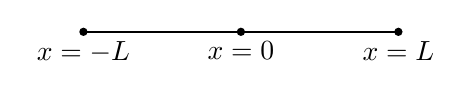
\begin{tikzpicture}
      \draw [thick] (-2, 0) -- (2, 0);
      \node [circ] at (0, 0) {};
      \node [below] at (0, 0) {$x = 0$};

      \node [circ] at (-2, 0) {};
      \node [below] at (-2, 0) {$x = -L$};

      \node [circ] at (2, 0) {};
      \node [below] at (2, 0) {$x = L$};
    \end{tikzpicture}
  \end{center}
  We have the initial conditions
  \[
    \phi(x, 0) = \Theta(x) =
    \begin{cases}
      1 & 0 < x < L\\
      0 & -L < x < 0
    \end{cases}
  \]
  and the boundary conditions
  \[
    \phi(-L, t) = 0,\quad \phi(L, t) = 1
  \]
  So we start with a step temperature, and then maintain the two ends at fixed temperatures $0$ and $1$.

  We are going to do separation of variables, but we note that all our boundary and initial conditions are inhomogeneous. This is not helpful. So we use a little trick. We first look for \emph{any} solution satisfying the boundary conditions $\phi_S(-L, t) = 0$, $\phi_S(L, t) = 1$. For example, we can look for time-independent solutions $\phi_S(x, t) = \phi_S(x)$. Then we need $\frac{\d^2 \phi_S}{\d x^2} = 0$. So we get
  \[
    \phi_S(x) = \frac{x + L}{2L}.
  \]
  By linearity, $\psi(x, t) = \phi(x, t) - \phi_s(x)$ obeys the heat equation with the conditions
  \[
    \psi(-L, t) = \psi(L, t) = 0,
  \]
  which is homogeneous! Our initial condition now becomes
  \[
    \psi(x, 0) = \Theta(x) - \frac{x + L}{2L}.
  \]
  We now perform separation of variables for
  \[
    \psi(x, t) = X(x) T(t).
  \]
  Then we obtain the equations
  \[
    T' = -\kappa \lambda T,\quad X' = - \lambda X.
  \]
  Then we have
  \[
    \psi(x, t) = \left[a\sin (\sqrt{\lambda} x) + b\cos (\sqrt{\lambda}x)\right] e^{-\kappa \lambda t}.
  \]
  Since initial condition is odd, we can eliminate all $\cos$ terms. Our boundary conditions also requires
  \[
    \lambda = \frac{n^2 \pi^2}{L^2}, \quad n = 1, 2, \cdots.
  \]
  So we have
  \[
    \phi(x, t) = \phi_s(x) + \sum_{n = 1}^\infty a_n \sin\left(\frac{n\pi x}{L}\right) \exp\left(-\frac{\kappa n^2 \pi^2}{L^2}t\right),
  \]
  where $a_n$ are the Fourier coefficients
  \[
    a_n = \frac{1}{L}\int_{-L}^L \left[\Theta(x) - \frac{x + L}{2L}\right] \sin\left(\frac{n\pi x}{L}\right)\;\d x = \frac{1}{n\pi}.
  \]
\end{eg}

\begin{eg}[Cooling of a uniform sphere]
  Once upon a time, Charles Darwin went around the Earth, looked at species, and decided that evolution happened. When he came up with his theory, it worked quite well, except that there was one worry. Was there enough time on Earth for evolution to occur? He knew well that the Earth started as a ball of molten rock, and obviously life couldn't have evolved when the world was still molten rock. So he would want to know how long it took for the Earth to cool down to its current temperature, and if that was sufficient for evolution to occur.

  We can, unsurprisingly, use the heat equation. We assume that at time $t = 0$, the temperature is $\phi_0$, the melting temperature of rock. We also assume that the space is cold, and we let the temperature on the boundary of Earth as $0$. We then solve the heat equation on a sphere (or ball), and see how much time it takes for Earth to cool down to its present temperature.

  We let $\Omega = \{(x, y, z) \in \R^3, r \leq R\}$, and we want a solution $\phi(r, t)$ of the heat equation that is spherically symmetric and obeys the conditions
  \begin{itemize}
    \item $\phi(R, t) = 0$
    \item $\phi(r, 0) = \phi_0$,
  \end{itemize}
  We can write the heat equation as
  \[
    \frac{\partial \phi}{\partial t} = \kappa \nabla^2 \phi = \frac{\kappa}{r^2}\frac{\partial}{\partial r}\left(r^2 \frac{\partial \phi}{\partial r}\right).
  \]
  Again, we do the separation of variables.
  \[
    \phi(r, t) = R(r) T(t).
  \]
  So we get
  \[
    T' = -\lambda^2 \kappa T,\quad \frac{\d}{\d r}\left(r^2 \frac{\d R}{\d r}\right) = -\lambda^2 r^2 R.
  \]
  We can simplify this a bit by letting $R(r) = \frac{S(r)}{r}$, then our radial equation just becomes
  \[
    S'' = -\lambda^2 S.
  \]
  We can solve this to get
  \[
    R(r) = A_\lambda \frac{\sin \lambda r}{r} + B_\lambda \frac{\cos \lambda r}{r}.
  \]
  We want a regular solution at $r = 0$. So we need $B_\lambda = 0$. Also, the boundary condition $\phi(R, t) = 0$ gives
  \[
    \lambda = \frac{n\pi}{R},\quad n = 1, 2, \cdots
  \]
  So we get
  \[
    \phi(r, t) = \sum_{n \in \Z} \frac{A_n}{r} \sin\left(\frac{n\pi r}{R}\right) \exp\left(\frac{-\kappa n^2 \pi^2 t}{R^2}\right),
  \]
  where our coefficients are
  \[
    A_n = (-1)^{n + 1}\frac{\phi_0 R}{n\pi}.
  \]
  We know that the Earth isn't just a cold piece of rock. There are still volcanoes. So we know many terms still contribute to the sum nowadays. This is rather difficult to work with. So we instead look at the temperature gradient
  \[
    \frac{\partial \phi}{\partial r} = \frac{\phi_0}{r} \sum_{n \in \Z} (-1)^{n + 1} \cos \left(\frac{n\pi r}{R}\right) \exp\left(\frac{-\kappa n^2 \pi^2 t}{R^2}\right) + \sin\text{stuff}.
  \]
  We evaluate this at the surface of the Earth, $R = r$. So we get the gradient
  \[
    \left.\frac{\partial\phi}{\partial r}\right|_R = -\frac{\phi_0}{R} \sum_{n\in \Z} \exp\left(-\frac{\kappa n^2 \pi^2 t}{R^2}\right) \approx \frac{\phi_0}{R} \int_{-\infty}^\infty \exp\left(-\frac{\kappa \pi y^2 t}{R^2}\right)\;\d y = \phi_0 \sqrt{\frac{1}{\pi \kappa t}}.
  \]
  So the age of the Earth is approximately
  \[
    t \approx \left(\frac{\phi_0}{V}\right)^2 \frac{1}{4\pi K},
  \]
  where
  \[
    V = \left.\frac{\partial \phi}{\partial r}\right|_R.
  \]
  We can plug the numbers in, and get that the Earth is 100 million years. This is not enough time for evolution.

  Later on, people discovered that fission of metals inside the core of Earth produce heat, and provides an alternative source of heat. So problem solved! The current estimate of the age of the universe is around 4 billion years, and evolution did have enough time to occur.
\end{eg}

\subsection{The wave equation}
Consider a string $x\in [0, L]$ undergoing small oscillations described by $\phi(x, t)$.
\begin{center}
  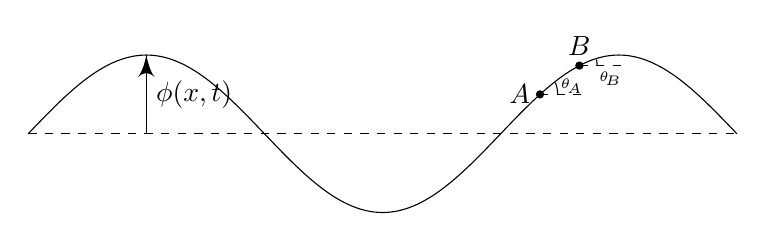
\begin{tikzpicture}[xscale=0.75]
    \draw (0, 0) sin (2, 1) cos (4, 0) sin (6, -1) cos (8, 0) sin (10, 1) cos (12, 0);
    \draw [dashed] (0, 0) -- (12, 0);

    \draw [->] (2, 0) -- (2, 1) node [pos=0.5, right] {$\phi(x, t)$};
    \node [circ] at (8.666, 0.5) {};
    \node [left] at (8.666, 0.5) {$A$};
    \node [circ] at (9.333, 0.866) {};
    \node [above] at (9.333, 0.866) {$B$};
    \draw [dashed] (8.666, 0.5) -- +(0.7, 0);
    \draw (8.666, 0.5) +(0.3, 0) arc(0:30:0.3);
    \node [right] at (8.85, 0.6) {\tiny$\theta\!_A$};

    \draw [dashed] (9.333, 0.866) -- +(0.7, 0);
    \draw (9.333, 0.866) +(0.3, 0) arc (0:15:0.3);
    \node [right] at (9.5, 0.7) {\tiny$\theta\!_B$};
  \end{tikzpicture}
\end{center} % improve
Consider two points $A$, $B$ separated by a small distance $\delta x$. Let $T_A$ ($T_B$) be the  outward pointing tension tangent to the string at $A$ ($B$). Since there is no sideways ($x$) motion, there is no net horizontal force. So
\[
  T_A\cos \theta_A = T_B \cos \theta_B = T.\tag{$*$}
\]
If the string has mass per unit length $\mu$, then in the vertical direction, Newton's second law gives
\[
  \mu \delta x \frac{\partial^2 \phi}{\partial t^2} = T_B \sin \theta_B - T_A \sin \theta_A.
\]
We now divide everything by $T$, noting the relation $(*)$, and get
\begin{align*}
  \mu \frac{\delta x}{T}\frac{\partial^2 \phi}{\partial t^2} &= \frac{T_B \sin \theta_B}{T_B\cos \theta_B} - \frac{T_A \sin \theta_A}{T_A \cos \theta_A}\\
  &= \tan \theta_B - \tan \theta_A\\
  &= \left.\frac{\partial\phi}{\partial x}\right|_B - \left.\frac{\partial\phi}{\partial x}\right|_A\\
  &\approx \delta x\frac{\partial^2 \phi}{\partial x^2}.
\end{align*}
Taking the limit $\delta x \to 0$ and setting $c^2 = T/\mu$, we have that $\phi(x, t)$ obeys the wave equation
\[
  \frac{1}{c^2} \frac{\partial^2 \phi}{\partial t^2} = \frac{\partial^2 \phi}{\partial x^2}.
\]
From IA Differential equations, we've learnt that the solution can be written as $f(x - ct) + g(x + ct)$. However, this does not extend to higher dimensions, but separation of variables does. So let's do that.

Assume that the string is fixed at both ends. Then $\phi(0, t) = \phi(L, t) = 0$ for all $t$. The we can perform separation of variables, and the general solution can then be written
\[
  \phi(x, t) = \sum_{n = 1}^\infty \sin\left(\frac{n \pi x}{L}\right)\left[A_n \cos\left(\frac{n \pi c t}{L}\right) + B_n \sin\left(\frac{n\pi ct}{L}\right)\right].
\]
The coefficients $A_n$ are fixed by the initial profile $\phi(x, 0)$ of the string, while the coefficients $B_n$ are fixed by the initial string velocity $\frac{\partial \phi}{\partial t} (x, 0)$. Note that we need \emph{two} sets of initial conditions, since the wave equation is second-order in time.

\subsubsection*{Energetics and uniqueness}
An oscillating string contains has some sort of \emph{energy}. The \emph{kinetic energy} of a small element $\delta x$ of the string is
\[
  \frac{1}{2}\mu \delta x\left(\frac{\partial \phi}{\partial t}\right)^2.
\]
The \emph{total kinetic energy} of the string is hence the integral
\[
  K(t) = \frac{\mu}{2}\int_0^L \left(\frac{\partial \phi}{\partial t}\right)^2 \;\d x.
\]
The string also has potential energy due to tension. The \emph{potential energy} of a small element $\delta x$ of the string is
\begin{align*}
  T\times \text{extension} &= T(\delta s - \delta x) \\
  &= T(\sqrt{\delta x^2 + \delta \phi^2} - \delta x)\\
  &\approx T\delta x\left(1 + \frac{1}{2}\left(\frac{\delta \phi}{\delta x}\right)^2 + \cdots\right) - T \delta x\\
  &= \frac{T}{2}\delta x \left(\frac{\delta \phi}{\delta x}\right)^2
\end{align*}
Hence the total potential energy of the string is
\[
  V(t) = \frac{\mu}{2}\int_0^L c^2 \left(\frac{\partial \phi}{\partial x}\right)^2 \;\d x,
\]
using the definition of $c^2$.

Using our series expansion for $\phi$, we get
\begin{align*}
  K(t) &= \frac{\mu \pi^2 c^2}{4L}\sum_{n = 1}^\infty n^2 \left[A_n \sin \left(\frac{n\pi c t}{L}\right) - B_n \cos \left(\frac{n\pi ct}{L}\right)\right]^2\\
  V(t) &= \frac{\mu\pi^2 c^2}{4L} \sum_{n = 1}^\infty n^2 \left[A_n \cos\left(\frac{n\pi ct}{L}\right) + B_n \sin\left(\frac{n\pi ct}{L}\right)\right]^2
\end{align*}
The \emph{total energy} is
\[
  E(t) = \frac{n\pi^2 c^2}{4L}\sum_{n = 1}^\infty n^2 (A_n^2 + B_n^2).
\]
What can we see here? Our solution is essentially an (infinite) sum of independent harmonic oscillators, one for each $n$. The period of the fundamental mode ($n = 1$) is $\frac{2\pi}{\omega} = 2\pi \cdot \frac{L}{\pi c} = \frac{2L}{c}$. Thus, averaging over a period, the average kinetic energy is
\[
  \bar K = \frac{c}{2L} \int_0^{2L/c} K(t)\;\d t = \bar V = \frac{c}{2L}\int_0^{2L/c} V(t)\;\d t = \frac{E}{2}.
\]
Hence we have an equipartition of the energy between the kinetic and potential energy.

The energy also allows us to prove a uniqueness theorem. First we show that energy is conserved in general.

\begin{prop}
  Suppose $\phi: \Omega \times [0, \infty) \to \R$ obeys the wave equation $\frac{\partial^2 \phi}{\partial t^2} = c^2 \nabla^2 \phi$ inside $\Omega \times (0, \infty)$, and is fixed at the boundary. Then $E$ is constant.
\end{prop}

\begin{proof}
  By definition, we have
  \[
    \frac{\d E}{\d t} = \int_\Omega \frac{\partial^2 \psi}{\partial t^2}\frac{\partial \psi}{\partial t} + c^2 \nabla \left(\frac{\partial \phi}{\partial t}\right)\cdot \nabla \phi \;\d V.
  \]
  We integrate by parts in the second term to obtain
  \[
    \frac{\d E}{\d t} = \int_\Omega \frac{\d \phi}{\d t}\left(\frac{\partial^2 \phi}{\partial t^2} - c^2 \nabla^2 \phi\right)\;\d V + c^2 \int_{\partial \Omega} \frac{\partial \phi}{\partial t}\nabla \phi \cdot \d S.
  \]
  Since $\frac{\partial^2 \phi}{\partial t^2} = c^2 \nabla^2 \phi$ by the wave equation, and $\phi$ is constant on $\partial \Omega$, we know that
  \[
    \frac{\d E_\phi}{\d t} = 0.
  \]
\end{proof}

\begin{prop}
  Suppose $\phi: \Omega \times [0, \infty) \to \R$ obeys the wave equation $\frac{\partial^2 \phi}{\partial t^2} = c^2 \nabla^2 \phi$ inside $\Omega \times (0, \infty)$, and obeys, for some $f, g, h$,
  \begin{enumerate}
    \item $\phi(x, 0) = f(x)$;
    \item $\frac{\partial \phi}{\partial t}(x, 0) = g(x)$; and
    \item $\phi|_{\partial \Omega\times [0, \infty)} = h(x)|_{\partial \Omega}$.
  \end{enumerate}
  Then $\phi$ is unique.
\end{prop}
\begin{proof}
  Suppose $\phi_1$ and $\phi_2$ are two such solutions. Then $\psi = \phi_1 - \phi_2$ obeys the wave equation
  \[
    \frac{\partial^2 \psi}{\partial t^2} = c^2 \nabla^2 \psi,
  \]
  and
  \[
    \psi|_{\partial \Omega \times [0, \infty)} = \psi|_{\Omega \times \{0\}} = \left.\frac{\partial \psi}{\partial t}\right|_{\Omega \times \{0\}} = 0.
  \]
  We let
  \[
    E_\psi(t) = \frac{1}{2}\int_\Omega \left[\left(\frac{\partial \psi}{\partial t}\right)^2 + c^2 \nabla \psi \cdot \nabla \psi\right] \;\d V.
  \]
  Then since $\psi$ obeys the wave equation with fixed boundary conditions. So $E_\psi$ is constant.

  Initially, at $t = 0$, we know that $\psi = \frac{\partial \psi}{\partial t} = 0$. So $E_\psi(0) = 0$. At time $t$, we must have
  \[
    E_\psi = \frac{1}{2}\int_\Omega \left(\frac{\partial \psi}{\partial t}\right)^2 + c^2 (\nabla \psi)\cdot (\nabla \psi) \;\d V = 0.
  \]
  Hence we must have $\frac{\partial \psi}{\partial t} = 0$. So $\psi$ is constant. Since it is $0$ at the beginning, it is always $0$.
\end{proof}

\begin{eg}
  Consider $\Omega = \{(x, y) \in \R^2, x^2 + y^2 \leq 1\}$, and let $\phi(r, \theta, t)$ solve
  \[
    \frac{1}{c^2}\frac{\partial^2 \phi}{\partial t^2} = \nabla^2 \phi = \frac{1}{r} \left(r \frac{\partial \phi}{\partial r}\right) + \frac{1}{r^2}\frac{\partial^2\phi}{\partial \theta^2},
  \]
  with the boundary condition $\phi|_{\partial \Omega} = 0$. We can imagine this as a drum, where the membrane can freely oscillate with the boundary fixed.

  Separating variables with $\phi(r, \theta, t) = T(t) R(r) \Theta(\theta)$, we get
  \[
    T'' = - c^2 \lambda T,\quad \Theta'' = -\mu \Theta,\quad r(R')' + (r^2\lambda - \mu)R = 0.
  \]
  Then as before, $T$ and $\Theta$ are both sine and cosine waves. Since we are in polars coordinates, we need $\phi(t, r, \theta + 2\pi) = \phi(t, r, \theta)$. So we must have $\mu = m^2$ for some $m \in \N$. Then the radial equation becomes
  \[
    r(rR')' + (r^2 \lambda - m^2) R = 0,
  \]
  which is Bessel's equation of order $m$. So we have
  \[
    R(r) = a_m J_m(\sqrt{\lambda} r) + b_m Y_m(\sqrt{\lambda} r).
  \]
  Since we want regularity at $r = 0$, we need $b_m = 0$ for all $m$. To satisfy the boundary condition $\phi|_{\partial \Omega} = 0$, we must choose $\sqrt{\lambda} = k_{mi}$, where $k_{mi}$is the $i$th root of $J_m$.

  Hence the general solution is
  \begin{align*}
    \phi(t, r, \theta) &= \sum_{i = 0}^\infty [A_{0i}\sin (k_{0i} ct) + B_{0i}\cos(k_{0i}ct)] J_0 (k_{0i}r)\\\
    &\quad\quad +\sum_{m = 1}^\infty\sum_{i = 0}^\infty [A_{mi}\cos (m \theta) + B_{mi}\sin (m\theta)]\sin k_{mi}ct J_m (k_{mi} r)\\
    &\quad\quad +\sum_{m = 1}^\infty\sum_{i = 0}^\infty [C_{mi}\cos (m \theta) + D_{mi}\sin (m\theta)]\cos k_{mi}ct J_m (k_{mi} r)
  \end{align*}
  For example, suppose we have the initial conditions $\phi(0, r, \theta) = 0$, $\partial_t \phi(0, r, \theta) = g(r)$. So we start with a flat surface and suddenly hit it with some force. By symmetry, we must have $A_{mi}, B_{mi}, C_{mi}, D_{mi} = 0$ for $m \not= 0$. If this does not seem obvious, we can perform some integrals with the orthogonality relations to prove this.

  At $t = 0$, we need $\phi = 0$. So we must have $B_{0i} = 0$. So we are left with
  \[
    \phi = \sum_{i = 0}^\infty A_{0i} \sin (k_{0i} ct) J_0(k_{0j}r).
  \]
  We can differentiate this, multiply with $J_0(k_{0j} r) r$ to obtain
  \[
    \int_0^1 \sum_{i = 0}^\infty k_{0i}c A_{0i}J_0(k_{0i}r) J_0(k_{0j} r)r\;\d r = \int_0^1 g(r) J_0(k_{0j}r)r \;\d r.
  \]
  Using the orthogonality relations for $J_0$ from the Example sheet, we get
  \[
    A_{0i} = \frac{2}{ck_{0i}} \frac{1}{[J_0'(k_{0i})]^2} \int_0^1 g(r)J_0(k_{0j} r) r\;\d r.
  \]
  Note that the frequencies come from the roots of the Bessel's function, and are not evenly spaced. This is different from, say, string instruments, where the frequencies are evenly spaced. So drums sound differently from strings.
\end{eg}

So far, we have used separation of variables to solve our differential equations. This is quite good, as it worked in our examples, but there are a few issues with it. Of course, we have the problem of whether it converges or not, but there is a more fundamental problem.

To perform separation of variables, we need to pick a good coordinate system, such that the boundary conditions come in a nice form. We were able to perform separation of variables because we can find some coordinates that fit our boundary conditions well. However, in real life, most things are not nice. Our domain might have a weird shape, and we cannot easily find good coordinates for it.

Hence, instead of solving things directly, we want to ask some more general questions about them. In particular, Kac asked the question ``can you hear the shape of a drum?'' --- suppose we know all the frequencies of the modes of oscillation on some domain $\Omega$. Can we know what $\Omega$ is like?

The answer is no. Fortunately, we get an affirmative answer if we restrict ourselves a bit. If we require $\Omega$ to be convex, and has a real analytic boundary, then yes! In fact, we have the following result: let $N(\lambda_0)$ be the number of eigenvalues less than $\lambda_0$. Then we can show that
\[
  4\pi^2 \lim_{\lambda_0 \to \infty} \frac{N(\lambda_0)}{\lambda_0} = \mathrm{Area}(\Omega).
\]

\section{Distributions}
\subsection{Distributions}
When performing separation of variables, we also have the problem of convergence as well. To perform separation of variables, we first find some particular solutions of the form, say, $X(x)Y(y)Z(z)$. We know that these solve, say, the wave equation. However, what we do next is take an \emph{infinite} sum of these functions. First of all, how can we be sure that this converges at all? Even if it did, how do we know that the sum satisfies the differential equation? As we have seen in Fourier series, an infinite sum of continuous functions can be discontinuous. If it is not even continuous, how can we say it is a solution of a differential equation?

Hence, at first people were rather skeptical of this method. They thought that while these methods worked, they only work on a small, restricted domain of problems. However, later people realized that this method is indeed rather general, as long as we allow some more ``generalized'' functions that are not functions in the usual sense. These are known as distributions.

To define a distribution, we first pick a class of ``nice'' test functions, where ``nice'' means we can do whatever we want to them (eg. differentiate, integrate etc.) A main example is the set of infinitely smooth functions with compact support on some set $K\subseteq \Omega$, written $C^{\infty}_{\mathrm{cpt}}(\Omega)$ or $D(\Omega)$. For example, we can have the bump function defined by
\[
  \phi(x) =
  \begin{cases}
    e^{-1/(1- x^2)} & |x| < 1\\
    0 & \text{otherwise}.
  \end{cases}
\]
\begin{center}
  \begin{tikzpicture}[scale=1.5]
    \draw [->] (-2, 0) -- (2, 0) node [right] {$x$};
    \draw [->] (0, -0.5) -- (0, 1);

    \draw [semithick, domain=-0.999:0.999, mblue] plot (\x, {exp (-1 / (1 - \x * \x))});
    \draw [semithick, mblue] (-1.5, 0) -- (-1, 0);
    \draw [semithick, mblue] (1, 0) -- (1.5, 0);
  \end{tikzpicture}
\end{center}
We now define a distribution $T$ to be a linear map $T:D(\Omega) \to \R$. For those who are doing IB Linear Algebra, this is the dual space of the space of (``nice'') real-valued functions. For $\phi \in D(\Omega)$, we often write its image under $T$ as $T[\phi]$.

\begin{eg}
  The simplest example is just an ordinary function that is integrable over any compact region. Then we define the distribution $T_f$ as
  \[
    T_f[\phi] = \int_\Omega f(x) \phi(x) \;\d x.
  \]
  Note that this is a linear map since integration is linear (and multiplication is commutative and distributes over addition). Hence every function ``is'' a distribution.
\end{eg}
Of course, this would not be interesting if we only had ordinary functions. The most important example of a distribution (that is not an ordinary function) is the Dirac delta ``function''.
\begin{defi}[Dirac-delta]
  The \emph{Dirac-delta} is a distribution defined by
  \[
    \delta[\phi] = \phi(0).
  \]
\end{defi}
By analogy with the first case, we often abuse notation and write
\[
  \delta[\phi] = \int_\Omega \delta(x) \phi(x) \;\d x,
\]
and pretend $\delta(x)$ is an actual function. Of course, it is not really a function, ie. it is not a map $\Omega \to \R$. If it were, then we must have $\delta(x) = 0$ whenever $x \not = 0$, since $\delta[\phi] = \phi(0)$ only depends on what happens at $0$. But then this integral will just give $0$ if $\delta(0) \in \R$. Some people like to think of this as a function that is zero anywhere and ``infinitely large'' everywhere else. Formally, though, we have to think of it as a distribution.

Although distributions can be arbitrarily singular, we can nonetheless define \emph{all} their derivatives, defined by
\[
  T'[\phi] = -T[\phi'].
\]
This is motivated by the case of the regular function, where we get, after integrating by parts,
\[
  \int_\Omega f'(x) \phi(x)\;\d x = -\int_\Omega f(x)\phi'(x) \;\d x,
\]
with no boundary terms since we have a compact support. Since $\phi$ is infinitely differentiable, we can take arbitrary derivatives of distributions.

So even though distributions can be crazy and singular, everything can be differentiated. This is good.

Generalized functions can occur as limits of sequences of normal functions. For example, the family of functions
\[
  G_n(x) = \frac{n}{\sqrt{\pi}} \exp(-n^2 x^2)
\]
are smooth for any finite $n$, and $G_n[\phi] \to \delta[\phi]$ for any $\phi$.
\begin{center}
  \begin{tikzpicture}
    \draw [->] (-3, 0) -- (3.25, 0) node [right] {$t$};
    \draw [->, use as bounding box] (0, 0) -- (0, 4) node [above] {$D$};

    \draw [semithick, mblue, domain=-3:3, samples = 100] plot (\x, { 1.6 * exp( - \x * \x)});
    \draw [semithick, morange, domain=-3:3, samples = 100] plot (\x, { 3.2 * exp( - 4 * \x * \x)});
  \end{tikzpicture}
\end{center}
It thus makes sense to define
\[
  \delta'(\phi) = -\delta[\phi'] = -\phi'(0),
\]
as this is the limit of the sequence
\[
  \lim_{n \to \infty}\int_\Omega G'_n(x) \phi(x)\;\d x.
\]
It is often convenient to think of $\delta(x)$ as $\lim\limits_{n \to \infty} G_n(x)$, and $\delta'(x) = \lim\limits_{n \to \infty} G'_n(x)$ etc, despite the fact that these limits do not exist as functions.

We can look at some properties of $\delta(x)$:
\begin{itemize}
  \item Translation:
    \[
      \int_{-\infty}^\infty \delta(x - a) \phi(x)\;\d x = \int_{-\infty}^\infty \delta(y) \phi(y + a)\;\d x.
    \]
  \item Scaling:
    \[
      \int_{-\infty}^\infty \delta(cx) \phi(x)\;\d x = \int_{-\infty}^\infty \delta(y) \phi\left(\frac{y}{c}\right) \frac{\d y}{|c|} = \frac{1}{|c|}\phi(0).
    \]
  \item These are both special cases of the following: suppose $f(x)$ is a continuously differentiable function with isolated simple zeros at $x_i$. Then near any of its zeros $x_i$, we have $f(x) \approx (x - x_i) \left.\frac{\partial f}{\partial x}\right|_{x_i}$. Then
    \begin{align*}
      \int_{-\infty}^\infty \delta(f(x)) \phi(x)\;\d x &= \sum_{i = 1}^n \int_{-\infty}^\infty \delta\left((x - x_i)\left.\frac{\partial f}{\partial x}\right|_{x_i}\right) \phi(x)\;\d x \\
      &= \sum_{i = 1}^n \frac{1}{|f'(x_i)|} \phi(x_i).
    \end{align*}
\end{itemize}
We can also expand the $\delta$-function in a basis of eigenfunctions. Suppose we live in the interval $[-L, L]$, and write a Fourier expansion
\[
  \delta(x) = \sum_{n \in \Z}\hat{\delta}_n e^{in\pi x/L}
\]
with
\[
  \hat{\delta}_n = \frac{1}{2L} \int_{-L}^L e^{in\pi x/L}\delta(x)\;\d x = \frac{1}{2L}
\]
So we have
\[
  \delta(x) = \frac{1}{2L} \sum_{n \in \Z} e^{in\pi x/L}.
\]
This \emph{does} make sense as a distribution. We let
\[
  S_N \delta(x) = \frac{1}{2L} \sum_{n = -N}^N e^{in \pi x/L}.
\]
Then
\begin{align*}
  \lim_{N \to \infty} \int_{-L}^L S_N \delta(x) \phi(x)\;\d x &= \lim_{N \to \infty} \frac{1}{2L}\int_{L}^L \sum_{n = -N}^N e^{in\pi x/L}\phi(x) \;\d x\\
  &= \lim_{N \to \infty} \sum_{n = -N}^N \left[\frac{1}{2L}\int_{-L}^L e^{in\pi x/L} \phi(x) \;\d x\right]\\
  &= \lim_{N\to \infty} \sum_{n = -N}^N \hat{\phi}_{-n}\\
  &= \lim_{N \to \infty}\sum_{n = -N}^N \hat{\phi}_n e^{in\pi 0/L}\\
  &= \phi(0),
\end{align*}
since the Fourier series of the smooth function $\phi(x)$ \emph{does} converge for all $x \in [-L, L]$.

We can equally well expand $\delta(x)$ in terms of any other set of orthonormal eigenfunctions. Let $\{y_n(x)\}$ be a complete set of eigenfunctions on $[a, b]$ that are orthogonal with respect to a weight function $w(x)$. Then we can write
\[
  \delta (x - \xi) = \sum_{n} c_n y_n(x),
\]
with
\[
  c_n = \int_a^b y_n^*(x) \delta(x - \xi) w(x)\;\d x = y_n^*(\xi) w(\xi).
\]
So
\[
  \delta(x - \xi) = w(\xi) \sum_n y_n^* (\xi) y_n(x) = w(x) \sum_n y_n^*(\xi) y_n(x),
\]
using the fact that
\[
  \delta(x - \xi) = \frac{w(\xi)}{w(x)} \delta(x - \xi).
\]
\subsection{Green's functions}
One of the main uses of the $\delta$ function is the Green's function. Suppose we wish to solve the 2nd order ordinary differential equation $\mathcal{L}y = f$, where $f(x)$ is a bounded forcing term, and $\mathcal{L}$ is a bounded differential operator, say
\[
  \mathcal{L} = \alpha(x) \frac{\partial^2}{\partial x^2} + \beta(x) \frac{\partial}{\partial x} + \gamma(x).
\]
As a first step, we try to find the Green's function for $\mathcal{L}$, which we shall write as $G(x, \xi)$, which obeys
\[
  \mathcal{L} G(x, \xi) = \delta(x - \xi).
\]
Given $G(x, \xi)$, we can then define
\[
  y(x) = \int_{a}^b G(x, \xi) f(\xi) \;\d \xi.
\]
Then we have
\[
  \mathcal{L}y = \int_a^b \mathcal{L} G(x, \xi) f(\xi)\;\d \xi = \int_a^b \delta(x - \xi) f(\xi) \;d\xi = f(x).
\]
We can formally say $y = \mathcal{L}^{-1} f$, and the Green's function shows that $\mathcal{L}^{-1}$ means an integral.

Hence if we can solve for Green's function, then we have solved the differential equation, at least in terms of an integral.

To find the Green's function $G(x, \xi)$ obeying the boundary conditions $G(a, \xi) = G(b, \xi) = 0$, first note that $\mathcal{L} G = 0$ for all $x \in [a, \xi) \cup (\xi, b]$, ie. everywhere except $\xi$ itself. Thus we must be able to expand it in a basis of solutions in these two regions.

Suppose $\{y_1(x), y_2(x)\}$ are a basis of solutions to $\mathcal{L}G = 0$ everywhere on $[a, b]$, with boundary conditions $y_1(a) = 0, y_2(b) = 0$. Then we must have
\[
  G(x, \xi) =
  \begin{cases}
    A(\xi) y_1(x) & a \leq x < \xi\\
    B(\xi) y_2(x) & \xi < x \leq b
  \end{cases}
\]
So we have a whole family of solutions. To fix the coefficients, we must decide how to join these solutions together over $x = \xi$.

If $G(x, \xi)$ were discontinuous at $x = \xi$, then $\partial_x G|_{x = \xi}$ would involve a $\delta$ function, while $\partial^2_x G|_{x = \xi}$ would involve the derivative of the $\delta$ function. This is not good, since nothing in $\mathcal{L}G = \delta(x - \xi)$ would balance a $\delta'$. So $G(x, \xi)$ must be everywhere continuous. Hence we require
\[
  A(\xi) y_1 (\xi) = B(\xi) y_2(\xi).\tag{$*$}
\]
Now integrate over a small region $(\xi - \varepsilon, \xi + \varepsilon)$ surrounding $\xi$. Then we have
\[
  \int_{\xi - \varepsilon}^{\xi + \varepsilon} \left[\alpha(x) \frac{\d^2 G}{\d x^2} + \beta(x) \frac{\d G}{\d x} + \gamma(x) G\right]\;\d x = \int_{\xi - \varepsilon}^{\xi + \varepsilon} \delta(x - \xi)\;\d x = 1.
\]
By continuity of $G$, we know that the $\gamma G$ term does not contribute. While $G'$ is discontinuous, it is still finite. So the $\beta G'$ term also does not contribute. So we have
\[
  \lim_{\varepsilon \to 0} \int_{\xi - \varepsilon}^{\xi + \varepsilon} \alpha G'' \;\d x = 1.
\]
We now integrate by parts to obtain
\[
  \lim_{\varepsilon \to 0} [\alpha G']^{\xi + \varepsilon}_{\xi - \varepsilon} + \int_{\xi - \varepsilon}^{\xi + \varepsilon} \alpha' G' \;\d x = 1.
\]
Again, by finiteness of $G'$, the integral does not contribute. So we know that
\[
  \alpha(\xi)\left(\left.\frac{\partial G}{\partial x}\right|_{\xi^+} - \left.\frac{\partial G}{\partial x}\right|_{\xi^-}\right) = 1
\]
Hence we obtain
\[
  B(\xi) y'_2 (\xi) - A(\xi) y_1'(\xi) = \frac{1}{\alpha(\xi)}.
\]
Together with $(*)$, we know that
\[
  A(\xi) = \frac{y_2(\xi)}{\alpha(\xi) W(\xi)},\quad B(\xi) = \frac{y_1(\xi)}{\alpha(\xi)W(\xi)},
\]
where $W$ is the \emph{Wronskian}
\[
  W = y_1 y_2' - y_2y_1'.
\]
Hence, we know that
\[
  G(x, \xi) = \frac{1}{\alpha(\xi)W(\xi)}
  \begin{cases}
    y_2(\xi) y_1(x) & a \leq x \leq \xi\\
    y_1(\xi) y_2(x) & \xi < x \leq b.
  \end{cases}
\]
Using the step function $\Theta$, we can write this as
\[
  G(x, \xi) = \frac{1}{\alpha(\xi)W(\xi)} [\Theta (\xi - x) y_2(\xi)y_1(x) + \Theta(x - \xi)y_1(\xi)y_2(x)].
\]
SO our general solution is
\begin{align*}
  y(x) &= \int_a^b G(x, \xi) f(\xi)\;\d \xi\\
  &= \int_a^b \frac{f(\xi)}{\alpha(\xi)W(\xi)} y_2(\xi) y_1(x)\;\d \xi + \int_a^x \frac{f(\xi)}{\alpha(\xi)W(\xi)}y_1(\xi) y_2(x)\;\d \xi.
\end{align*}

\begin{eg}
  Consider
  \[
    \mathcal{L}y= -y'' - y = f
  \]
  for $x \in (0, 1)$ with $y(0) = y(1) = 0$. We choose our basis solution to satisfy $y'' = -y$ as $\{\sin x, \sin (1 - x)\}$. Then we can compute the Wronskian
  \[
    W(x) = -\sin x \cos(1 - x) - \sin (1 - x) \cos x = -\sin 1.
  \]
  Our Green's function is
  \[
    G(x, \xi) = \frac{1}{\sin 1}[\Theta(\xi - x) \sin (1 - \xi) \sin x + \Theta(x - \xi) \sin \xi \sin (1 - x)].
  \]
  Hence we get
  \[
    y(x) = \sin x \int_{x}^1 \frac{\sin (1 - \xi)}{ \sin 1}f(\xi) \;\d \xi + \sin(1 - x)\int_0^x \frac{\sin \xi}{\sin 1}f(\xi)\;\d \xi.
  \]
\end{eg}

\begin{eg}
  Suppose we have a string with mass per unit length $\mu(x)$ and held under a tension $T$. In the presence of gravity, Newton's second law gives
  \[
    \mu\frac{\partial^2 y}{\partial t^2} = T \frac{\partial^2 y}{\partial x^2} + \mu g.
  \]
  We look for the steady state solution $\dot{y} = 0$ shape of the string, assuming $y(0, t) = y(L, t) = 0$. So we get
  \[
    \frac{\partial^2 y}{\partial x^2} = -\frac{\mu(x)}{T}g.
  \]
  We look for a Green's function obeying
  \[
    \frac{\partial^2 y}{\partial x^2} = - \delta(x - \xi).
  \]
  This can be interpreted as the contribution of a pointlike mass located at $x = \xi$.
  \begin{center}
    \begin{tikzpicture}
      \draw [gray] (-0.5, 0) -- (4.5, 0);
      \node [circ] at (0, 0) {};
      \node [circ] at (4, 0) {};
      \draw (0, 0) -- (1, -1) -- (4, 0);
      \node [circ] at (1, -1) {};
      \node [above] at (0, 0) {$0$};
      \node [above] at (4, 0) {$L$};
      \node [above] at (1, 0) {$\xi$};
      \draw [dashed] (1, 0) -- (1, -1);
      \draw [->] (1, -1) -- +(0, -0.5) node [below] {$y$};
    \end{tikzpicture}
  \end{center}
  The homogeneous equation $y'' = 0$ gives
  \[
    y = Ax + B(x - L).
  \]
  So we get
  \[
    G(x, \xi) =
    \begin{cases}
      A(\xi x) & 0 \leq x < \xi\\
      B(\xi)(x - L) & \xi < x \leq L.
    \end{cases}
  \]
  Continuity at $x = \xi$ gives
  \[
    A(\xi)\xi = B(\xi) (\xi -L).
  \]
  The jump condition on the derivative gives
  \[
    A(\xi) - B(\xi) = 1.
  \]
  We can solve these to get
  \[
    A(\xi) = \frac{\xi - L}{L},\quad B(\xi) = \frac{\xi}{L}.
  \]
  Hence the Green's function is
  \[
    G(x, \xi) = \frac{\xi - L}{L} \Theta(\xi - x) + \frac{\xi}{L}(x - L) \Theta(x - \xi).
  \]
  Notice that $\xi$ is always less that $L$. So the first term has a negative slope; while $\xi$ is always positive, so the second term has positive slope.

  For the general case, we can just substitute this into the integral. We can also first think that we have many pointlike particles $m_i$ at small separations $\Delta x$ along the string. So we get
  \[
    g(x) = \sum_{i = 1}^n G(x, x_i) \frac{m_i g}{T},
  \]
  and in the limit $\Delta x \to 0$ and $n \to \infty$, we get
  \[
    g(x) \to \frac{g}{T} \int_0^L G(x, \xi) \mu(\xi)\;\d \xi.
  \]
\end{eg}
\subsection{Green's functions for initial value problems}
Consider $\mathcal{L}y = f(t)$ subject to $y(t = t_0) = 0$ and $y'(t = t_0) = 0$. So instead of having two boundaries, we have one boundary and restrict both the value and the derivative at this boundary.

As before, let $y_1(t), y_2(t)$ be \emph{any} basis of solutions to $\mathcal{L} y = 0$. The Green's function obeys
\[
  \mathcal{L}(G) = \delta(t - \tau).
\]
We can write our Green's function as
\[
  G(t, \tau) =
  \begin{cases}
    A(\tau) y_1(t) + B(\tau) y_2(t) & t_0 \leq t < \tau\\
    C(\tau) y_1(t) + D(\tau) y_2(t) & t > \tau.
  \end{cases}
\]
Our initial conditions require that
\[
  \begin{pmatrix}
    y_1(t_0) & y_2(t_0)\\
    y_1'(t_0) & y_2'(t_0)
  \end{pmatrix}
  \begin{pmatrix}
    A\\
    B
  \end{pmatrix}
  =
  \begin{pmatrix}
    0\\0
  \end{pmatrix}
\]
However, we know that the matrix is non-singular (by definition of $y_1, y_2$ being a basis). So we must have $A, B = 0$ (which makes sense, since $G = 0$ is obviously a solution for $t_0 \leq t < \tau$).

Our continuity and jump conditions now require
\begin{align*}
  0 &= C(\tau) t_1(t) + D(\tau) y_2(t)\\
  \frac{1}{\alpha(t\tau)} &= C(\tau) y_1'(\tau)  + D(\tau) y_2'(\tau).
\end{align*}
We can solve this to get $C(\tau)$ and $D(\tau)$. Then we get
\[
  y(t) = \int_{t_0}^\infty G(t, \tau) f(\tau)\;\d \tau = \int_{t_0}^t G(t, \tau) f(\tau) \;\d \tau,
\]
since we know that when $\tau > t$, the Green's function $G(t, \tau) = 0$. Thus the solution $y(t)$ depends on the forcing term term $f$ only for times $ < t$. This expresses causality!

\begin{eg}
  For example, suppose we have $\ddot{y} + y = f(t)$ with $f(0) = \dot{y}(0) = 0$. Then we have
  \[
    G(t, \tau) = \Theta(t - \tau) [C(\tau) \cos(t - \tau) + D(\tau) \sin (t - \tau)]
  \]
  for some $C(\tau), D(\tau)$. The continuity and jump conditions gives $D(\tau) = 1, C(\tau) = 0$. So we get
  \[
    G(t, \tau) = \Theta(t - \tau) \sin t(\tau).
  \]
  So we get
  \[
    y(t) = \int_0^t \sin (t - \tau) f(\tau) \;\d \tau.
  \]
\end{eg}
\end{document}
